% !TEX TS-program = xelatex
% !BIB program = bibtex
% !TeX spellcheck = ru_RU

% About magic macroses see also
% https://tex.stackexchange.com/questions/78101/

% По умолчанию используется шрифт 14 размера. Если нужен 12-й шрифт, уберите опцию [14pt]
\documentclass[14pt, russian, table, dvipsnames]{matmex-diploma-custom}


\usepackage{float}
% \usepackage[linesnumbered,lined]{algorithm2e}
\usepackage{pgfplots}
% \usepackage{makecell}
\usepackage{tikz}
\usepackage{multirow}
\usepackage{url}
\usetikzlibrary{shapes.geometric, shapes.misc, arrows.meta, positioning, fit, calc, matrix, backgrounds}

% Команда для имён файлов и идентификаторов кода: моноширинный шрифт + разрешённые
% переносы строк по символам _, ., / (на основе механизма пакета url).
\DeclareUrlCommand{\code}{\urlstyle{tt}}


\def\bbljan{Jan.}
\def\bblfeb{Feb.}
\def\bblmar{Mar.}
\def\bblapr{Apr.}
\def\bblmay{May}
\def\bbljun{Jun.}
\def\bbljul{Jul.}
\def\bblaug{Aug.}
\def\bblsep{Sep.}
\def\bbloct{Oct.}
\def\bblnov{Nov.}
\def\bbldec{Dec.}


\pgfplotsset{compat=1.18}
\begin{document}

\input{title.tex}
\maketitle
\setcounter{tocdepth}{2}
\tableofcontents

% !TeX spellcheck = ru_RU
% !TEX root = vkr.tex

\section*{Введение}
\thispagestyle{withCompileDate}

Морфометрия~--- количественное описание формы биологических объектов~--- является одним из ключевых инструментов таксономии и экологии~\cite{Bookstein1991,DrydenMardia1998}.
Несмотря на развитый аппарат статистического анализа, получение исходных данных по-прежнему остаётся ручной или полуавтоматической операцией: исследователь вручную обводит контур каждого объекта в растровом редакторе и вручную снимает измерения.
При сериях из десятков и сотен образцов это занимает значительное время и вносит субъективную погрешность, особенно когда измерения ведут несколько человек~\cite{Bookstein1998}.

Задача осложняется при работе с морфологически сложными объектами.
Листья мхов рода \textit{Sphagnum}~--- экологически значимых эдификаторов торфяных болот и тундровых сообществ~\cite{ClymoHayward1982,Rydin2006}~--- состоят из одного слоя клеток, могут быть прозрачными и иметь неоднородные, рваные края.
Существующие программы автоматической «обрисовки» контуров (например, tpsDIG~\cite{Rohlf2021}) требуют хорошо контрастированных объектов без инородных включений и не справляются с такими объектами.

С технической точки зрения проблема состоит в отсутствии инструмента, объединяющего в едином рабочем цикле нейросетевую сегментацию, интерактивную коррекцию результата и автоматическое извлечение морфометрических параметров с экспортом в табличный формат.
Появление foundation-моделей сегментации~--- в частности, Segment Anything Model (SAM)~\cite{Kirillov2023} и её облегчённой версии MobileSAM~\cite{Zhang2023}~--- открывает возможность строить такой инструмент без необходимости собирать размеченные обучающие данные.
Настоящая работа направлена на решение описанной проблемы.

Работа имеет следующую структуру.
В разделе~\ref{sec:task} сформулированы цель, задачи и требования к разрабатываемой системе.
В разделе~\ref{sec:relatedworks} проведён обзор существующих инструментов и обоснован выбор модели сегментации.
В разделе~\ref{sec:solution} описаны архитектура и реализация приложения.
В разделе~\ref{sec:experiment} приведены результаты сравнения с ручной разметкой и апробации.
Заключение содержит выводы и направления дальнейшего развития системы.

% !TeX spellcheck = ru_RU
% !TEX root = vkr.tex

\section{Постановка задачи}
\label{sec:task}

\subsection{Цель и задачи работы}

Работа выполняется в интересах лаборатории Гербарий ГБС РАН, сотрудники которой проводят морфометрический анализ листьев мохообразных (в первую очередь мхов рода \textit{Sphagnum}).

Рабочий процесс биолога включает два принципиально разных этапа.
Первый~--- \textit{отбор образцов}: на каждом изображении присутствуют несколько листьев,
и исследователь выбирает те из них, которые пригодны для измерений.
«Хороший» лист~--- целый, с неповреждёнными краями, типичной для вида формы,
расположен изолированно и не перекрывается с другими объектами.
Листья с рваными или нечёткими краями, артефактами препарирования,
атипичной морфологией или сильным перекрытием исключаются.
Критерии отбора субъективны, определяются целями конкретного исследования
и требуют экспертной оценки биолога; формализовать их в виде алгоритма невозможно.
Второй этап~--- \textit{сегментация и измерение} отобранных листьев~---
представляет собой технически однообразную ручную работу, которая при сериях из десятков
и сотен образцов занимает значительное время и вносит субъективную погрешность.

\textbf{Цель работы}~--- разработать настольное приложение, автоматизирующее цикл
«загрузка изображений → сегментация → ручная коррекция → параметрические измерения → экспорт»,
пригодное для использования без специальных вычислительных ресурсов на рабочих станциях биологической лаборатории.

Для достижения цели поставлены следующие \textbf{задачи}:
\begin{enumerate}
    \item Проанализировать существующие программные решения для сегментации и морфометрии биологических объектов и обосновать выбор модели сегментации.
    \item Сформулировать требования к системе совместно с заказчиком~--- сотрудниками лаборатории Гербарий ГБС РАН.
    \item Спроектировать архитектуру приложения и реализовать его.
    \item Реализовать алгоритм параметрических измерений (длина, поперечные профили ширины).
    \item Сравнить результаты автоматической сегментации с ручной разметкой биологов и провести апробацию системы.
\end{enumerate}

\textbf{Практическая значимость} работы состоит в сокращении времени, затрачиваемого на получение морфометрических данных, и в повышении воспроизводимости измерений за счёт стандартизованного алгоритма обработки.


% !TeX spellcheck = ru_RU
% !TEX root = vkr.tex

\section{Обзор существующих решений}
\label{sec:relatedworks}

\subsection{Инструменты для морфометрии и сегментации изображений}

Задача получения морфометрических данных с изображений биологических объектов решается несколькими классами инструментов.

\textbf{ImageJ / FIJI}~\cite{Schindelin2012} является стандартом де-факто в биологических лабораториях.
Пакет предоставляет широкий набор инструментов для ручного обведения контуров и измерений,
а также плагины для полуавтоматической пороговой сегментации (Threshold, Wand tool, Trainable Weka).
Применительно к рассматриваемой задаче у FIJI выявлен ряд ограничений.
Во-первых, пороговая сегментация требует ручной настройки порогов под каждую серию снимков
и не справляется с прозрачными объектами и неоднородным фоном~--- типичными для препаратов листьев Sphagnum.
Плагин Trainable Weka Segmentation позволяет использовать машинное обучение,
однако требует ручной разметки обучающих областей для каждого нового типа объектов.
Во-вторых, рабочий процесс в FIJI фрагментирован: сегментация, коррекция, измерения
и экспорт выполняются разными инструментами, что требует экспертных знаний
и увеличивает число ручных операций.
В-третьих, FIJI не предоставляет встроенного инструмента для профильного анализа вдоль
главной оси объекта с автоматическим определением направления оси~---
поперечные сечения исследователь расставляет вручную, что вносит субъективность в измерения.

\textbf{tpsDIG2}~\cite{Rohlf2021}~--- специализированный инструмент для геометрической морфометрии,
позволяющий расставлять landmarks и строить контуры (outlines).
Требует хорошо контрастированных объектов без инородных включений и неоднородных краёв.
Листья Sphagnum с рваными краями и прозрачной текстурой плохо поддаются автоматической «обрисовке».

\textbf{PlantCV}~\cite{Fahlgren2015}~--- открытая Python-библиотека для анализа изображений растений.
Поддерживает пакетную обработку и разнообразные морфометрические функции (скелетизацию, измерение площади,
периметра, длины). Не имеет графического интерфейса, требует написания скриптов,
опирается на пороговые методы и морфологические операции без нейросетевой сегментации.

\textbf{Labelme / CVAT / Label Studio}~--- инструменты ручной разметки изображений,
позволяющие строить полигональные аннотации. Предназначены для создания обучающих наборов данных,
а не для морфометрии; не выполняют измерений.

\subsection{Сравнительный анализ}

Для сравнения выбраны критерии, непосредственно влияющие на трудоёмкость
морфометрической обработки серий гербарных снимков.

\begin{table}[H]
\centering
\caption{Сравнение существующих инструментов по ключевым критериям}
\label{tab:related}
\resizebox{\textwidth}{!}{%
\begin{tabular}{lcccccccc}
\hline
\textbf{Инструмент}
  & \textbf{\shortstack{ИИ-сегм.\\без обуч.\\данных}}
  & \textbf{\shortstack{Работа на\\сложных\\объектах}}
  & \textbf{\shortstack{Единый\\pipeline}}
  & \textbf{\shortstack{Ручная\\коррекция}}
  & \textbf{\shortstack{Профильный\\анализ\\по оси}}
  & \textbf{\shortstack{Стандарт.\\вывод}}
  & \textbf{\shortstack{Batch}}
  & \textbf{\shortstack{Без\\GPU}} \\
\hline
ImageJ / FIJI    & --    & $\pm$ & -- & + & -- & -- & $\pm$ & + \\
tpsDIG2          & --    & --    & -- & + & -- & $\pm$ & -- & + \\
PlantCV          & --    & $\pm$ & -- & -- & -- & + & +  & + \\
Labelme / CVAT   & $\pm$ & +     & -- & + & -- & -- & $\pm$ & + \\
\textbf{Разраб. система} & \textbf{+} & \textbf{+} & \textbf{+} & \textbf{+} & \textbf{+} & \textbf{+} & \textbf{+} & \textbf{+} \\
\hline
\multicolumn{9}{l}{\small \textbf{+}~--- поддерживается; $\pm$~--- частично / требует ручной настройки; \textbf{--}~--- не поддерживается} \\
\end{tabular}}
\end{table}

Сравнение показывает, что ни одно из рассмотренных решений не покрывает
полный рабочий цикл биолога в рамках одного приложения.
Наиболее близким аналогом является FIJI, однако его возможности применительно к задаче
ограничены по нескольким ключевым направлениям.

\textit{Сегментация сложных объектов.}
Встроенные инструменты FIJI (пороговая сегментация, Wand) рассчитаны на контрастные объекты.
Листья мохообразных с прозрачной клеточной структурой и рваными краями
существенно снижают качество автоматической обрисовки, вынуждая пользователя
выполнять значительный объём ручной правки.

\textit{Единый рабочий цикл.}
В FIJI сегментация, измерения и экспорт реализованы разными плагинами
и требуют переключения между инструментами и ручного переноса данных.
В разрабатываемой системе весь цикл~--- загрузка, сегментация, коррекция,
измерения, экспорт~--- выполняется в одном окне приложения без переключения контекста.

\textit{Стандартизированный профильный анализ.}
FIJI позволяет измерять ширину листа, но направление оси и точки сечения
задаются пользователем вручную для каждого образца.
Разрабатываемая система автоматически определяет главную ось методом PCA
и вычисляет ширину в фиксированных относительных точках ($0.125, 0.25, \ldots, 0.875$),
обеспечивая воспроизводимые и сопоставимые между собой профили для любой серии изображений.

\subsection{Выбор модели сегментации}

Ключевым техническим решением при разработке системы является выбор метода сегментации.
Ниже рассмотрены три класса подходов и обоснован итоговый выбор.

\subsubsection*{Требование интерактивности и проблема отбора образцов}

Прежде чем сравнивать подходы к сегментации, необходимо учесть ключевую особенность
рабочего процесса биологов-морфометристов.
На каждом изображении присутствует несколько листьев, и не все они пригодны для измерений.
Биолог отбирает «хорошие» листья~--- целые, с неповреждёнными краями, типичной для вида формы,
расположенные изолированно и не перекрывающиеся с другими объектами.
Листья с рваными краями, артефактами препарирования или атипичной морфологией исключаются.

Этот отбор по своей природе субъективен: критерии зависят от целей конкретного исследования,
вида и индивидуального опыта исследователя.
Попытка формализовать «хорошесть» листа в виде числовых порогов (площадь, компактность контура,
степень выпуклости) даёт лишь грубое приближение и требовала бы отдельной экспериментальной
валидации на реальном материале~--- задача, выходящая за рамки настоящей работы.
Таким образом, \textit{полностью автоматический} pipeline «обнаружить все листья → сегментировать →
измерить» не отвечает требованиям заказчика: он не позволяет исключить непригодные образцы
без участия эксперта.

Отсюда следует принципиальное требование к архитектуре системы:
\textbf{эксперт должен участвовать в отборе}, а система~--- снять с него трудоёмкую часть работы.
Идеальная модель сегментации в данном контексте~--- та, в которой
\textit{сам акт выбора листа и его сегментация совмещены в одно действие}:
исследователь указывает на нужный лист, система немедленно строит маску.

\subsubsection*{Классические алгоритмы компьютерного зрения}

Классические методы~--- пороговая сегментация, морфологические операции, алгоритм GrabCut,
watershed~--- не требуют обучающих данных и работают на любом CPU.
Однако они не удовлетворяют сформулированному выше требованию по двум причинам.
Во-первых, их применимость ограничена качеством входного материала:
листья Sphagnum могут быть практически прозрачными и иметь рваные края~---
именно те свойства, при которых пороговые методы дают фрагментированные маски
с пропусками в области прозрачных клеток.
Во-вторых, они не обеспечивают интерактивного отбора: алгоритм не знает,
\textit{какой именно} объект на изображении нужен биологу.

\subsubsection*{Специализированные нейросетевые модели (U-Net и аналоги)}

Архитектуры типа U-Net~\cite{Ronneberger2015} демонстрируют высокую точность сегментации биомедицинских изображений
при наличии размеченного обучающего набора данных.
В данном случае такого набора не существует: гербарная коллекция ГБС РАН содержит
тысячи образцов нескольких видов рода \textit{Sphagnum}, ни один из которых
не был ранее сегментирован в машиночитаемом формате.
Сбор репрезентативной обучающей выборки потребовал бы значительных трудозатрат
самих биологов~--- той самой ручной работы, которую требуется автоматизировать.
Помимо этого, обученная модель сегментирует все объекты подходящего класса на изображении,
не предоставляя механизма для интерактивного указания конкретного листа.

\subsubsection*{Foundation-модели сегментации: SAM и MobileSAM}

Segment Anything Model (SAM)~\cite{Kirillov2023}~--- foundation-модель сегментации от Meta AI,
обученная на датасете из более чем 1~млрд масок.
Ключевое свойство SAM~--- способность сегментировать произвольный объект
по интерактивным подсказкам (точки, ограничивающий прямоугольник) \textit{без дообучения на конкретном домене}.

SAM органично решает проблему отбора образцов: один клик по телу листа одновременно
является и выбором нужного объекта экспертом, и достаточной подсказкой для построения маски.
Биолог просто не кликает на «плохие» листья~--- и они автоматически исключаются из анализа.
Такой интерфейс не требует отдельного шага отбора и не накладывает на исследователя
никакой дополнительной когнитивной нагрузки по сравнению с тем, что он и так делает мысленно.

Базовая версия SAM имеет существенное ограничение для настольного приложения:
image encoder на основе ViT-H содержит 632~М параметров и требует GPU для приемлемой скорости работы.

\textbf{MobileSAM}~\cite{Zhang2023} решает эту проблему: тяжёлый encoder заменён
на компактный ViT-T ($\approx$5.7~М параметров), обученный методом knowledge distillation
на выходах оригинального SAM encoder.
Размер checkpoint~--- 39~МБ против 2.6~ГБ у ViT-H SAM.
Авторы показывают, что на задачах prompt-based сегментации качество MobileSAM
сопоставимо с оригиналом~\cite{Zhang2023}, при этом на CPU среднего рабочего компьютера
модель генерирует маску за 1--3~с~--- приемлемо для интерактивной работы.

\subsubsection*{Итог}

MobileSAM выбран в качестве модели сегментации по совокупности факторов:
\begin{itemize}
    \item не требует обучающих данных и обобщается на новые классы объектов;
    \item интерактивный prompt-based интерфейс естественно совмещает отбор образцов и сегментацию в одно действие;
    \item справляется с морфологически сложными объектами (прозрачные клетки, рваные края);
    \item работает на CPU, не требует GPU;
    \item умещается в дистрибутив настольного приложения (39~МБ).
\end{itemize}
SAM и MobileSAM не имеют собственного GUI и средств морфометрии~---
именно их интеграция в единый pipeline с интерактивной коррекцией и параметрическими измерениями
и составляет основной вклад разрабатываемой системы.

% !TeX spellcheck = ru_RU
% !TEX root = vkr.tex

\section{Разработка приложения}
\label{sec:solution}

\subsection{Требования к системе}
\label{sec:requirements}

Требования сформулированы совместно с консультантом (м.н.с.\ лаборатории Гербарий ГБС РАН, Шкурко~А.~В.)
на основе технического задания.

\subsubsection*{Требования}

\begin{itemize}
    \item Автоматическое распознавание формы листа и построение полигональной маски контура.
    \item Определение длины и ширины полигона.
    \item Расстановка точек вдоль перпендикуляров к главной оси с заданным шагом (например, $\frac{1}{2}$ или $\frac{1}{4}$ длины листа).
    \item Просмотр исходного изображения и маски на экране.
    \item Возможность задать масштабный коэффициент ($1~\text{пиксель} = \ldots~\text{мм}$) для вывода измерений в физических единицах.
    \item Экспорт результатов в табличный формат (CSV / Excel).
    \item Пакетная обработка серий изображений.
    \item Возможность ручной корректировки автоматически построенной маски.
    \item Режим автоматической сегментации и параметрических измерений: построение масок всех объектов без участия пользователя, автоматический отбор корректных листьев и запуск измерений.
\end{itemize}

\subsubsection*{Нефункциональные требования}

\begin{itemize}
    \item Работоспособность на стандартных рабочих станциях без выделенного GPU (инференс всех моделей на CPU). При наличии GPU приложение должно автоматически задействовать его для ускорения без дополнительной настройки.
    \item Время отклика модели сегментации не более 1~с на одно изображение в интерактивном режиме.
    \item Время обработки одного изображения не более 10~с в автоматическом режиме.
    \item Поддержка форматов JPEG, PNG, TIFF.
    \item Воспроизводимость результатов: одни и те же входные данные и подсказки дают одинаковый вывод.
    \item Единый формат хранения масок (PNG) и измерений (CSV / XLSX) для последующей статистической обработки.
\end{itemize}

\subsection{Архитектура приложения}
\label{sec:architecture}

Приложение реализовано на языке Python с использованием фреймворка PyQt6 для графического
интерфейса и библиотеки PyTorch для инференса MobileSAM. Исходный код опубликован по адресу
\url{https://github.com/pavelrubanov/segmentation_system}.

Кодовая база разделена на три слоя (рис.~\ref{fig:architecture}):

\begin{itemize}
    \item \textbf{Ядро (\code{src/core/}).} Вычислительные модули, не зависящие от UI:
          обёртка над MobileSAM, конвейер предобработки маски и канонизации листа,
          алгоритм параметрических измерений, общий конвейер пакетной обработки
          и экспорт результатов.
    \item \textbf{Интерфейс (\code{src/ui/}).} Окна и элементы интерфейса PyQt6:
          навигационное окно, окно интерактивной сегментации, общие компоненты
          пакетных диалогов и точки входа в пакетные режимы.
    \item \textbf{Классификатор (\code{classifier/}).} Изолированный пакет с собственными
          зависимостями: фиксированный экстрактор признаков MobileNetV3-Small и
          обучаемый XGBoost (подробности~--- в разделе~\ref{sec:classifier}).
\end{itemize}

\begin{figure}[H]
\centering
\begin{tikzpicture}[
    font=\footnotesize,
    layer/.style ={rectangle, draw, thick, rounded corners=4pt,
                   align=center, inner sep=10pt, fill=gray!4,
                   minimum width=5.6cm, minimum height=1.6cm},
    title/.style ={font=\bfseries\footnotesize},
    sub/.style   ={font=\scriptsize, color=black!70},
    weights/.style={rectangle, draw, dashed, rounded corners=2pt,
                    minimum height=0.55cm, font=\scriptsize, inner sep=4pt,
                    fill=white},
    arr/.style   ={->, >=Stealth, thick},
    lbl/.style   ={font=\scriptsize\itshape, inner sep=1pt},
]

% =====  UI layer (top)  =====
\node[layer] (uibox) at (0,0) {%
    {\bfseries\footnotesize UI (PyQt6) \textemdash{} \texttt{src/ui/}}\\[2pt]
    {\scriptsize\itshape окна, элементы интерфейса, диалоги пакетных режимов}};

% =====  Core layer (middle)  =====
\node[layer, below=1.2cm of uibox] (corebox) {%
    {\bfseries\footnotesize Ядро \textemdash{} \texttt{src/core/}}\\[2pt]
    {\scriptsize\itshape сегментация, канонизация, измерения, экспорт}};

% =====  Classifier layer (right of core)  =====
\node[layer, right=2.6cm of corebox, minimum width=4.4cm] (clbox) {%
    {\bfseries\footnotesize Классификатор}\\[1pt]
    {\bfseries\footnotesize\texttt{classifier/}}\\[2pt]
    {\scriptsize\itshape отбор корректных листьев}};

% =====  External: weights  =====
\node[weights, below=1.0cm of corebox.south]
    (sam) {\texttt{models/mobile\_sam.pt}};
\node[weights, below=1.0cm of clbox.south]
    (mdl) {\texttt{models/model\_<type>.pkl}};

% =====  Arrows  =====
\draw[arr] (uibox.south)   -- node[lbl, right]{использует} (corebox.north);
\draw[arr] (corebox.east)  -- node[lbl, above]{загружает}  (clbox.west);
\draw[arr] (sam.north)     -- (corebox.south);
\draw[arr] (mdl.north)     -- (clbox.south);

\end{tikzpicture}
\caption{Архитектура приложения: три независимых слоя и веса моделей,
подгружаемые на старте}
\label{fig:architecture}
\end{figure}

Точка входа~--- \code{src/main.py}: загружает веса MobileSAM, создаёт единственный
экземпляр \texttt{Predictor} (синглтон, общий для всех режимов) и открывает главное
окно навигации (рис.~\ref{fig:main_menu}). Из него доступны три режима:
интерактивная сегментация (раздел~\ref{sec:interactive}), параметрические
измерения по готовым фрагментам (раздел~\ref{sec:measure}) и автоматическая
сегментация и параметрические измерения (раздел~\ref{sec:auto_mode}).

\begin{figure}[H]
    \centering
    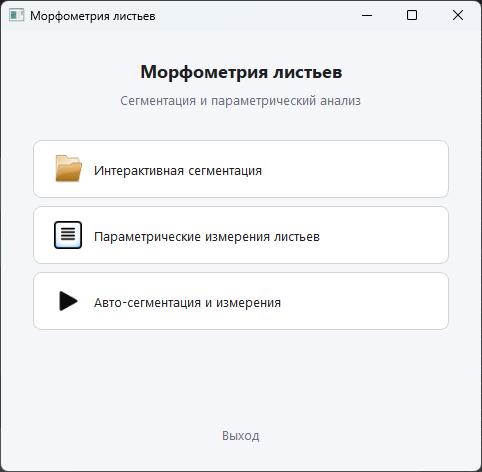
\includegraphics[width=0.5\linewidth]{figures/main_menu.png}
    \caption{Главное меню приложения}
    \label{fig:main_menu}
\end{figure}

Оба пакетных режима реализованы поверх общего конвейера обработки с подключаемыми
источниками фрагментов (см.\ раздел~\ref{sec:measure}).

\textbf{Конвенция имён файлов.} Все три источника артефактов~--- ручная сегментация
(раздел~\ref{sec:interactive}), автоматическая сегментация и параметрические
измерения (раздел~\ref{sec:auto_mode}) и
пользовательский ввод~--- порождают и потребляют файлы по единому шаблону:
\code{{stem}_leaf_crop_{idx:04d}.png} для фрагмента,
\code{{stem}_mask_{idx:04d}.png} для маски и \code{{crop_stem}_vis.png} для
визуализации измерений. Реализация и Qt-фильтры сосредоточены в модуле
\code{file_naming.py}, что позволяет смешивать в одной папке результаты разных
источников и переиспользовать их между режимами без отдельной конвертации.

\subsection{Интерактивная сегментация}
\label{sec:interactive}

Интерактивный режим (окно \texttt{SegmentationWindow}) реализует основной сценарий
работы биолога: эксперт самостоятельно выбирает листья на изображении, а система
строит маску по подсказке и при необходимости даёт инструменты ручной коррекции
(рис.~\ref{fig:segmentation_window}). Типовой рабочий цикл показан на
рис.~\ref{fig:activity}.

\begin{figure}[H]
    \centering
    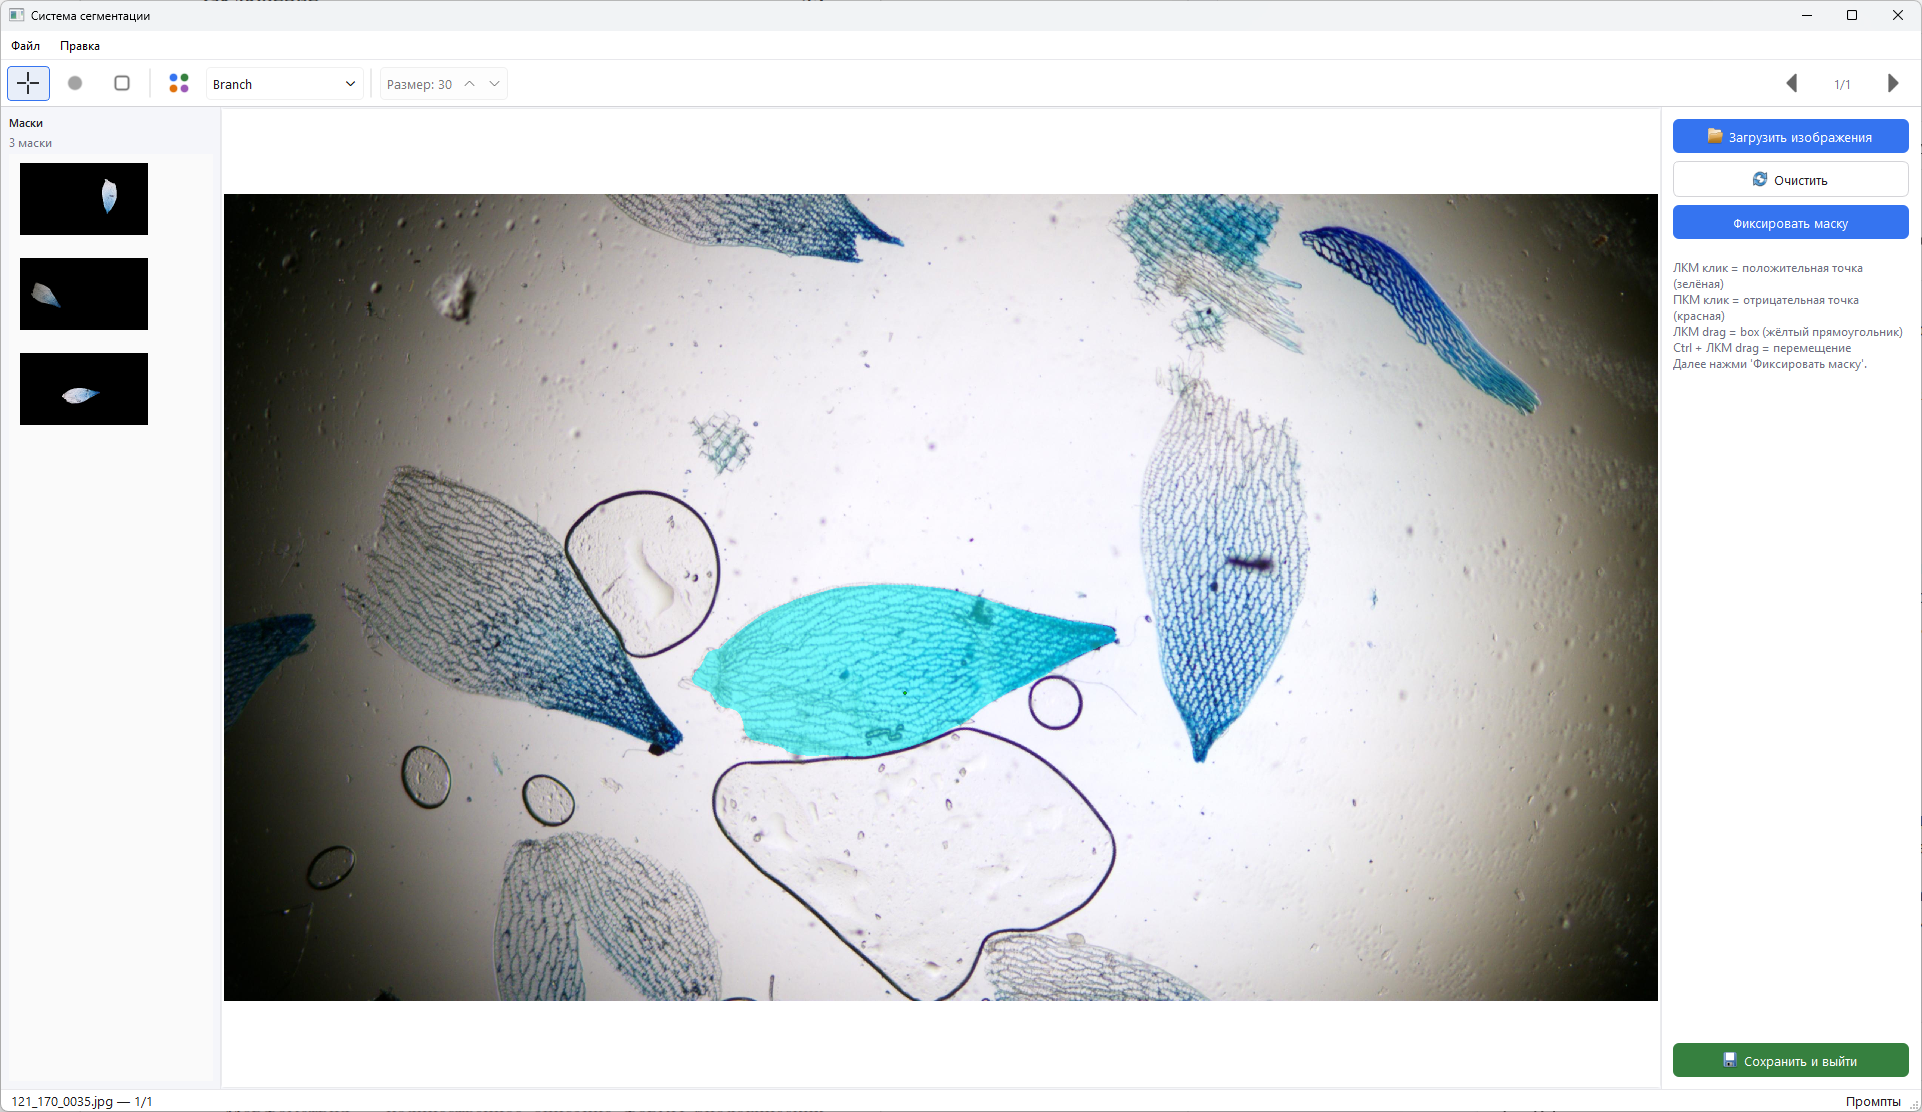
\includegraphics[width=0.95\linewidth]{figures/segmentation_canvas.png}
    \caption{Окно интерактивной сегментации}
    \label{fig:segmentation_window}
\end{figure}

\textbf{Загрузка серии и навигация.} Окно работает с серией изображений.
Загрузка набора файлов выполняется по нажатию кнопки <<Загрузить>> в боковой
панели или через пункт меню <<Файл~$\to$~Загрузить изображения>> (Ctrl+O):
выбранные снимки добавляются в очередь обработки и проходятся последовательно.
Перемещение между ними выполняется кнопками <<вперёд>> и <<назад>> в панели
инструментов; для каждого изображения сохраняется собственный буфер масок,
что позволяет накопить разметку по всей серии за один сеанс работы.

\textbf{Холст и режимы работы.} Центральный элемент интерфейса~--- \texttt{SegmentationCanvas}
на основе \texttt{QGraphicsView} с поддержкой зума к курсору и панорамирования
(\texttt{Ctrl + ЛКМ}). Холст имеет два режима. В режиме \emph{подсказок} клики
левой и правой кнопкой мыши задают позитивные и негативные опорные точки, а
перетаскивание ЛКМ~--- ограничивающий прямоугольник; после каждого изменения
автоматически вызывается \texttt{Predictor.predict}, и над изображением отображается
полупрозрачная маска. В режиме \emph{редактирования} ЛКМ работает кистью, а ПКМ~---
ластиком; диаметр кисти регулируется ползунком в панели инструментов в диапазоне $1\ldots200$~пикселей.
Маска хранится в виде ARGB-слоя (\texttt{QImage Format\_ARGB32}); переключение между
режимами не теряет промежуточный результат.

\textbf{Буфер масок.} Подтверждённые маски попадают в список \texttt{MasksBuffer}
(левая панель). Для каждой маски сохраняются два файла~--- собственно бинарная
маска и RGB-фрагмент, прошедший канонизацию (раздел~\ref{sec:pipeline}); при
выходе из окна они копируются в выбранную пользователем директорию.

\textbf{Кнопка авто-сегментации.} В панели инструментов доступна кнопка
автоматической сегментации текущего изображения~--- она запускает в фоновом
потоке тот же конвейер, что и режим автоматической сегментации и параметрических измерений
(шаги 1--4 раздела~\ref{sec:auto_mode}) для выбранного в панели типа листа. В буфер
добавляются все найденные корректные листья (рис.~\ref{fig:autosegment_result})~---
эксперту остаётся при необходимости скорректировать ошибочные маски и
доразметить пропущенные.

\begin{figure}[H]
    \centering
    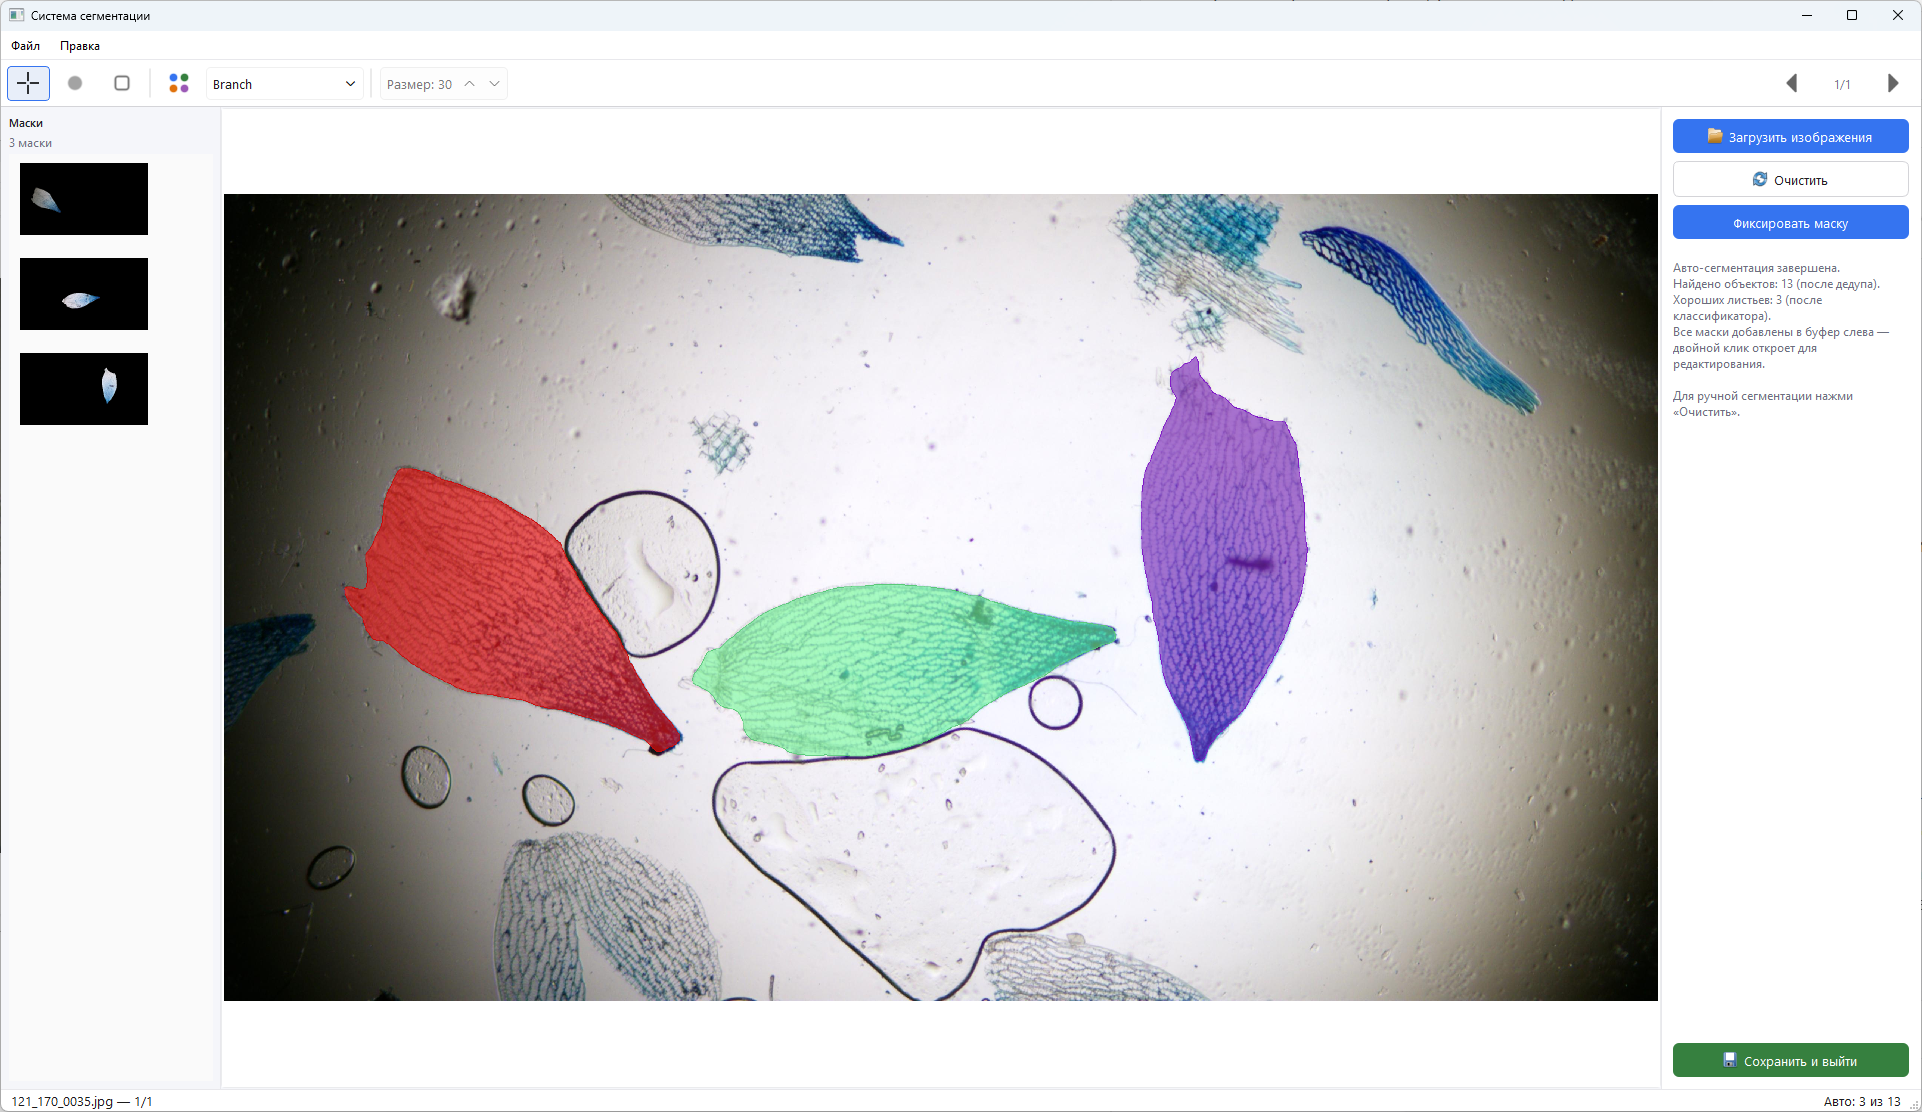
\includegraphics[width=0.95\linewidth]{figures/segmentation_canvas_autosegment_result.png}
    \caption{Результат нажатия кнопки авто-сегментации: на холсте отображены
    только листья, прошедшие классификатор отбора}
    \label{fig:autosegment_result}
\end{figure}

\begin{figure}[H]
\centering
\begin{tikzpicture}[
    font=\footnotesize,
    node distance=0.55cm,
    action/.style={rectangle, draw, rounded corners=3pt, align=center,
                   minimum width=4.8cm, minimum height=0.75cm, fill=white},
    decision/.style={diamond, draw, align=center, inner sep=1pt,
                     minimum width=1.0cm, fill=white},
    arr/.style={->, >=Stealth, thick},
    label/.style={font=\scriptsize, inner sep=1pt},
]

\node[draw, circle, fill=black, minimum size=0.28cm] (start) {};

\node[action,  below=of start]       (load)       {Загрузить папку с изображениями};
\node[action,  below=of load]        (nav)        {Перейти к следующему изображению};
\node[action,  below=of nav]         (click)      {Кликнуть на лист\\(positive point / bbox)};
\node[action,  below=of click]       (sam)        {\textit{[система]} Построить маску (MobileSAM)};
\node[decision,below=of sam]         (ok)         {Маска\\точная?};
\node[action,  below=of ok]          (save)       {\textit{[система]} Сохранить маску в буфер};
\node[decision,below=of save]        (moreleaves) {Ещё листья\\на изображении?};
\node[decision,below=of moreleaves]  (moreimages) {Ещё\\изображения?};
\node[action,  below=of moreimages]  (savebuf)    {Сохранить буфер масок\\и канонизированных фрагментов\\в выбранную папку};

\node[draw, circle, fill=black, minimum size=0.28cm,
      below=of savebuf] (end) {};
\node[draw, circle, minimum size=0.38cm] at (end) {};

\node[action, right=1.8cm of ok] (edit) {Исправить маску\\(кисть / ластик)};

\draw[arr] (start) -- (load);
\draw[arr] (load)  -- (nav);
\draw[arr] (nav)   -- (click);
\draw[arr] (click) -- (sam);
\draw[arr] (sam)   -- (ok);

\draw[arr] (ok)       -- node[label, left]{да} (save);
\draw[arr] (ok.east)  -- node[label, above]{нет} (edit.west);
\draw[arr] (edit.south) |- (save.east);

\draw[arr] (save) -- (moreleaves);

\draw[arr] (moreleaves) -- node[label, left]{нет} (moreimages);
\draw[arr] (moreleaves.west) -- ++(-2.0,0) node[label, above left]{да}
           |- (click.west);

\draw[arr] (moreimages) -- node[label, left]{нет} (savebuf);
\draw[arr] (moreimages.west) -- ++(-3.0,0) node[label, above left]{да}
           |- (nav.west);

\draw[arr] (savebuf) -- (end);

\end{tikzpicture}
\caption{Диаграмма активностей: рабочий цикл пользователя в интерактивном режиме}
\label{fig:activity}
\end{figure}

\subsection{Канонизация листа}
\label{sec:pipeline}

Маска, полученная сегментирующей моделью или ручной коррекцией, ориентирована
произвольно и может содержать мелкие артефакты~--- отдельные пиксели и
внутренние дыры. Перед измерениями и классификацией её приводят к стандартному
\emph{каноническому} виду: главная ось листа расположена вертикально, апекс
направлен вверх, фон обнулён, а контур очищен от артефактов
(рис.~\ref{fig:pipeline_stages}).

В этом виде фрагмент используется во всех последующих этапах обработки: на
канонических фрагментах работает алгоритм параметрических измерений
(раздел~\ref{sec:measure}), на них же обучается и применяется классификатор
отбора (глава~\ref{sec:classifier_chapter}); кроме того, канонический фрагмент
встраивается в визуализации и таблицы экспорта.

\begin{figure}[H]
    \centering
    \begin{tabular}{c@{\hspace{0.2cm}}c@{\hspace{0.2cm}}c@{\hspace{0.2cm}}c@{\hspace{0.2cm}}c}
        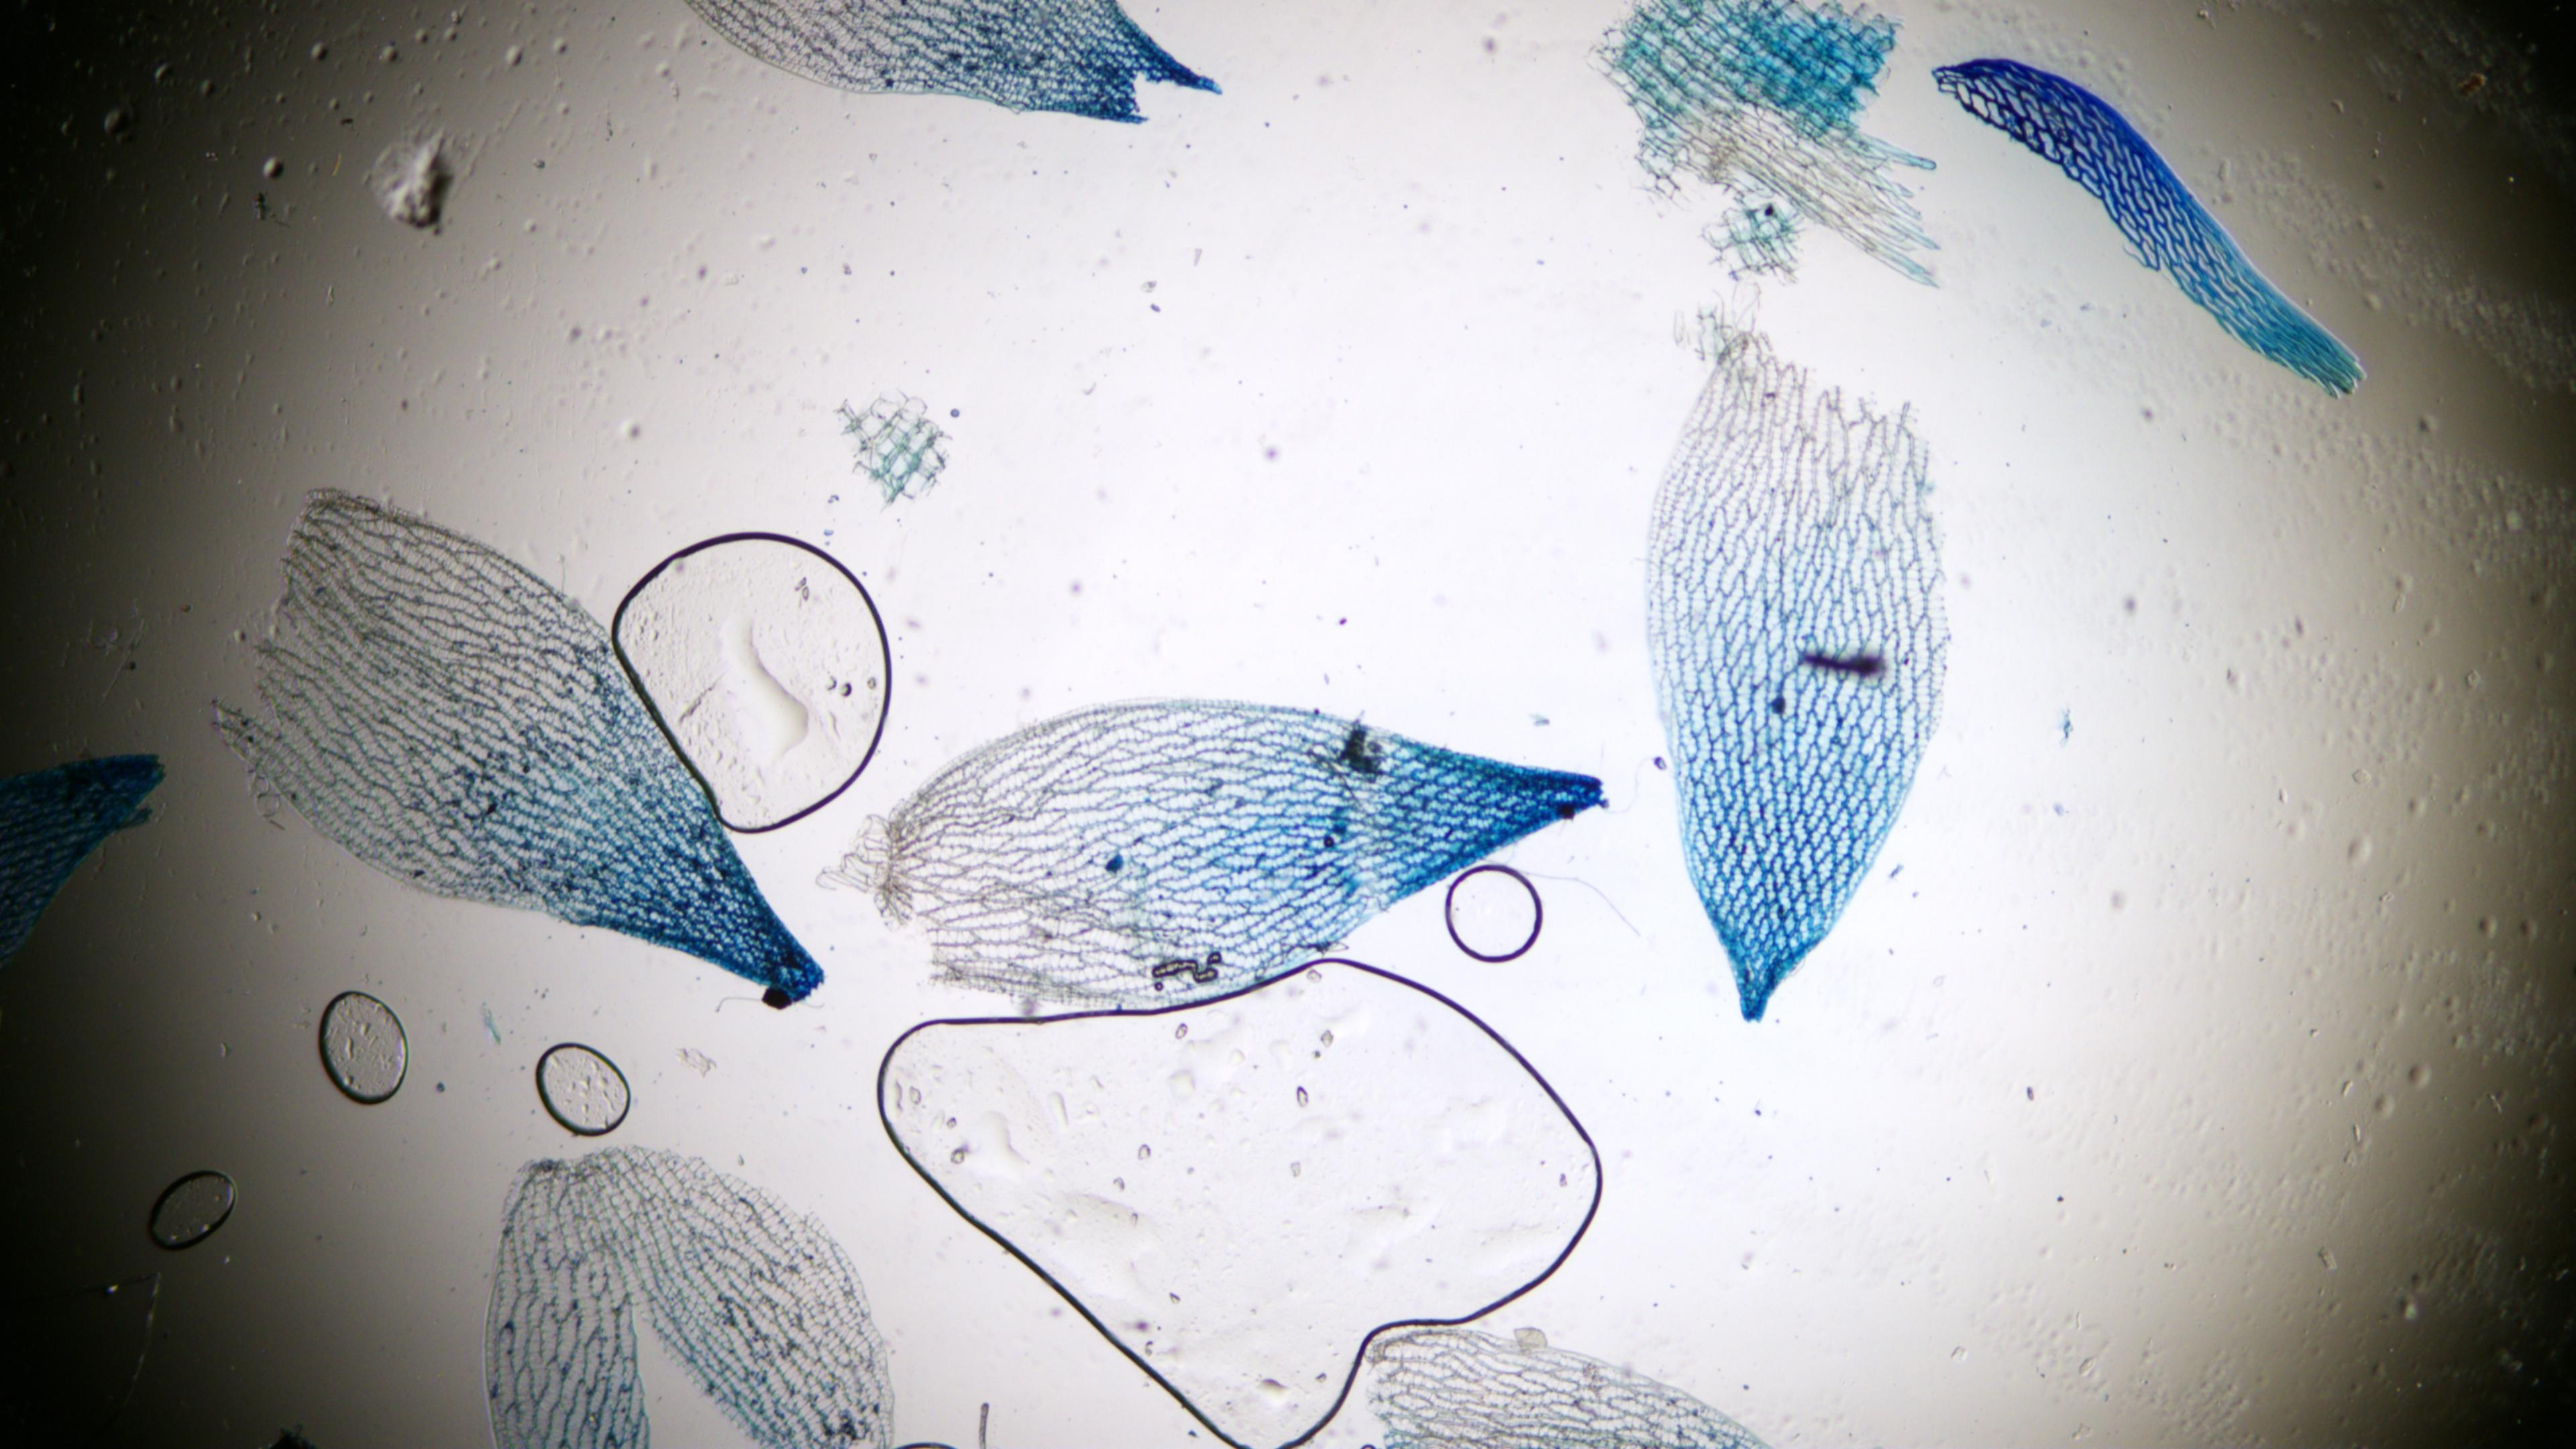
\includegraphics[height=2.8cm]{figures/121_170_0035.jpg} &
        \raisebox{1.2cm}{\Large$\to$} &
        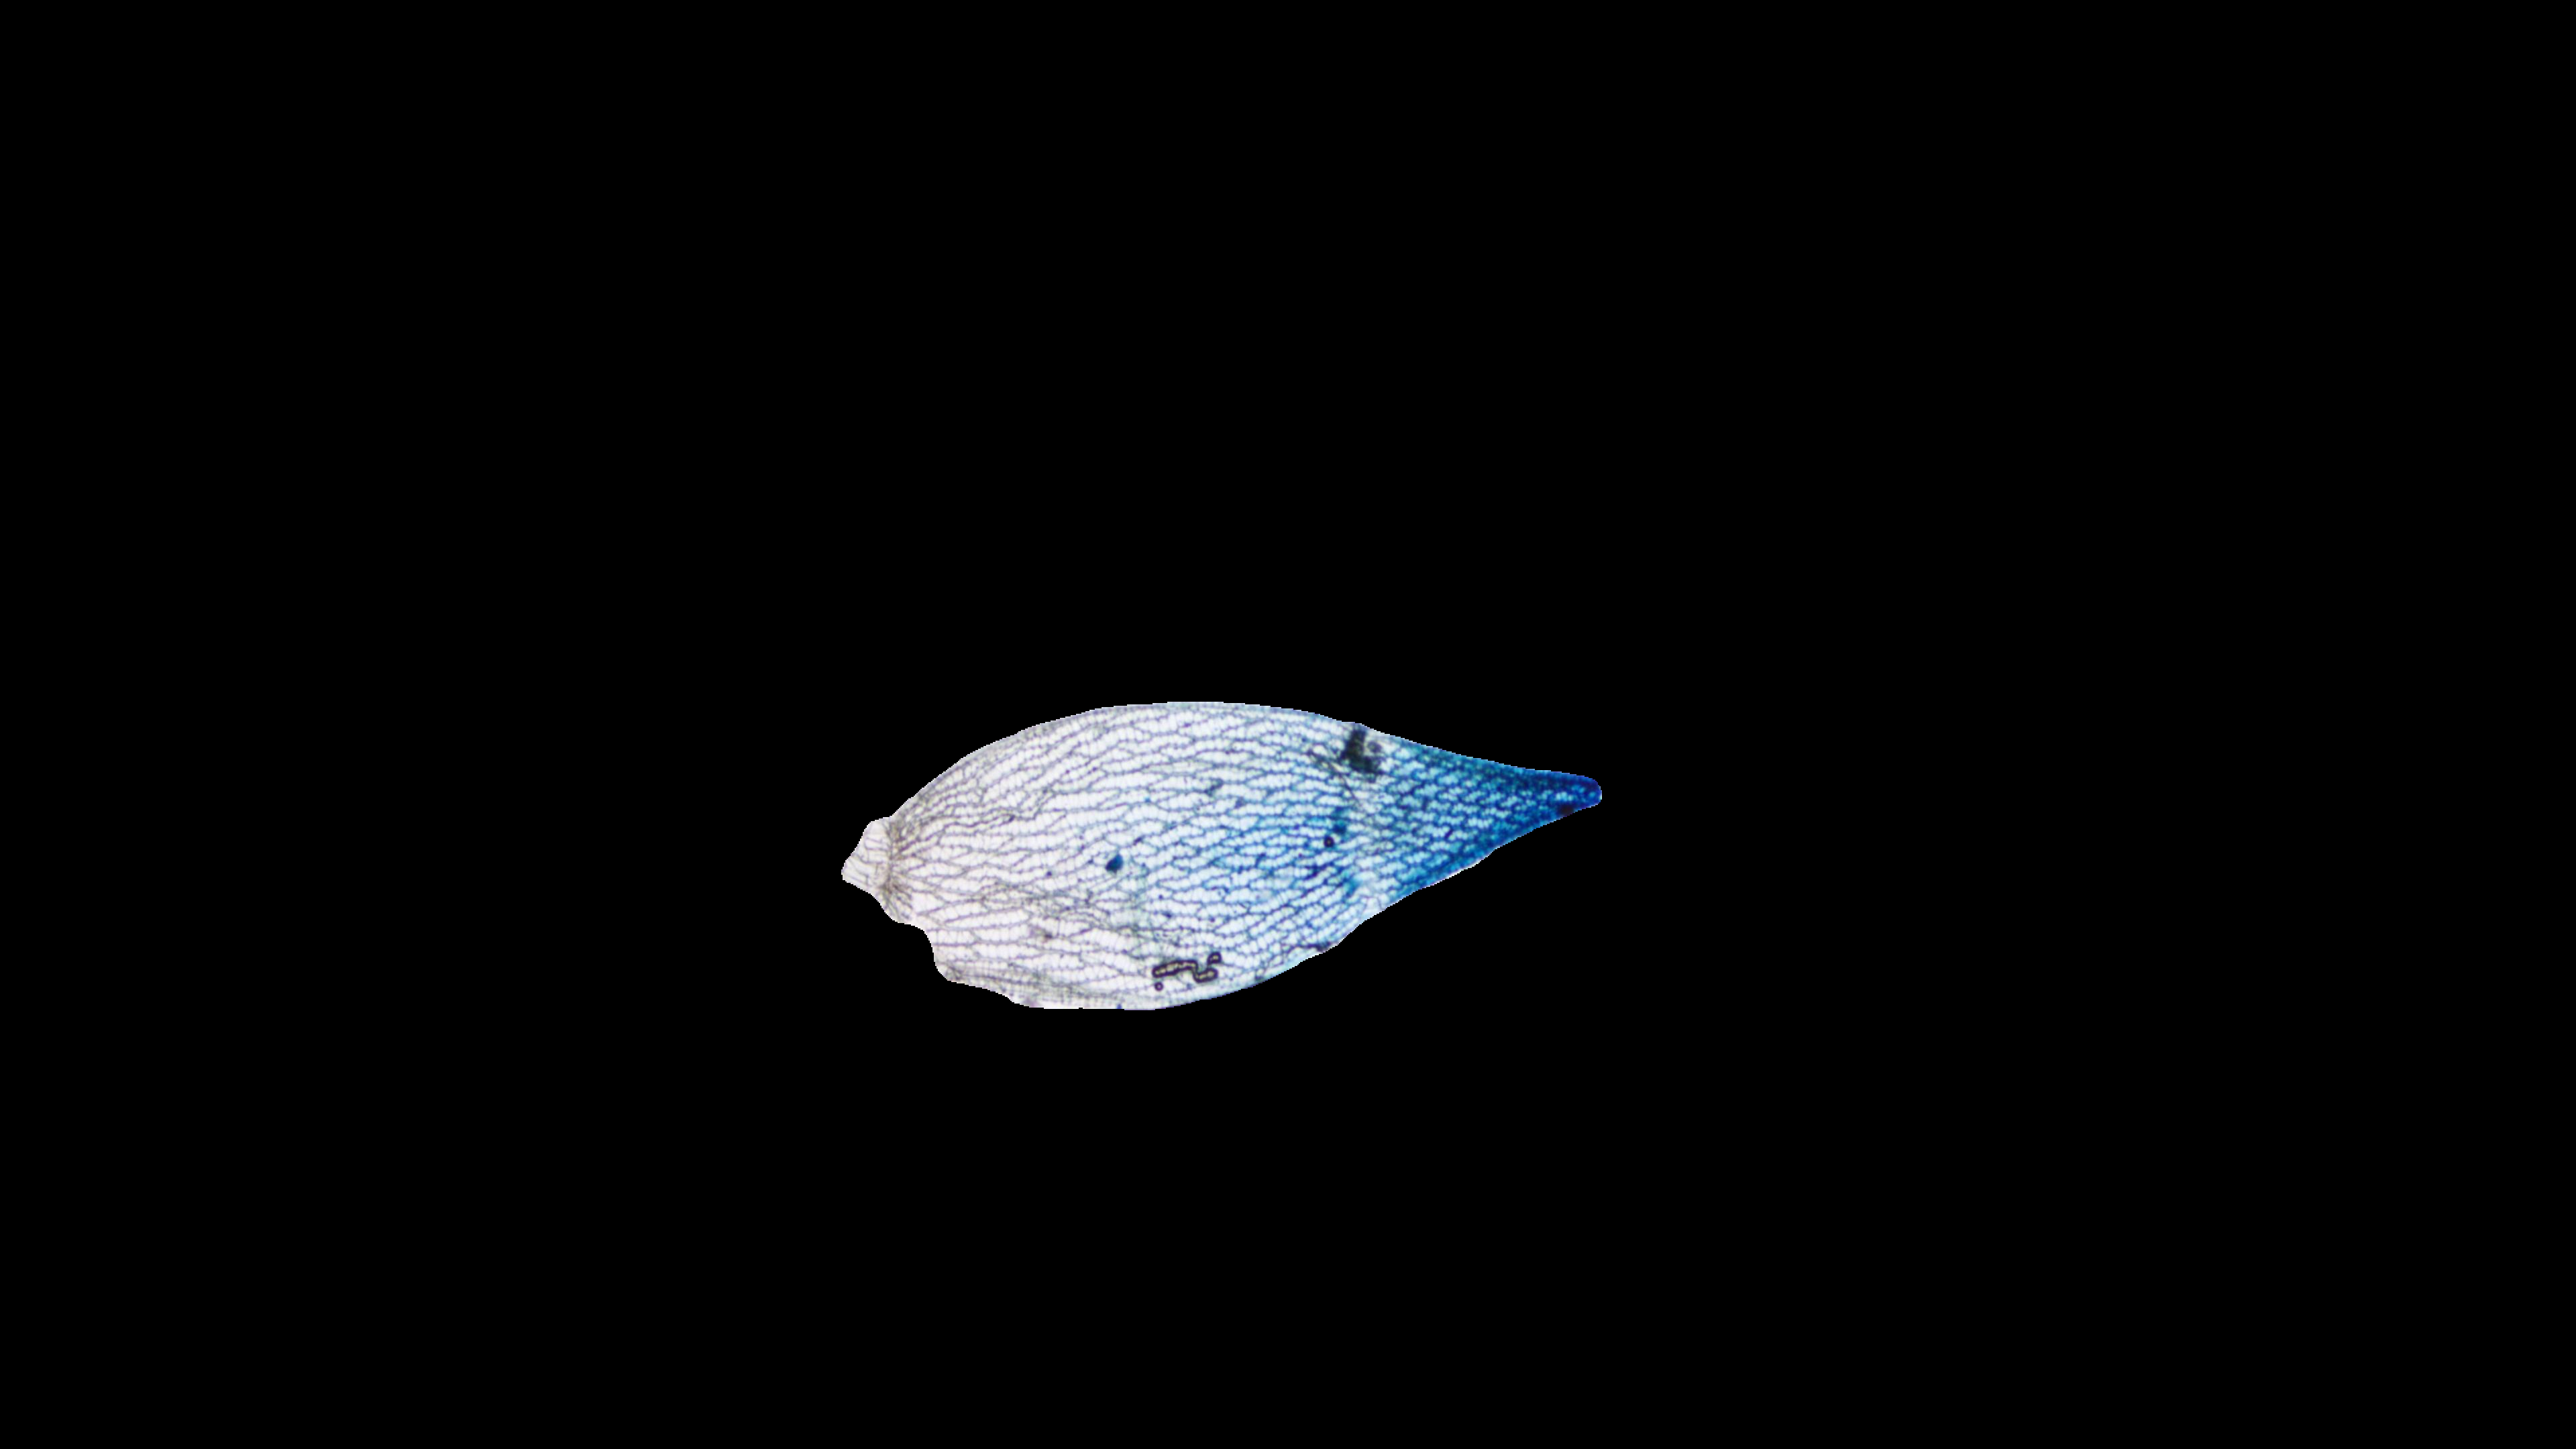
\includegraphics[height=2.8cm]{figures/121_170_0035_mask_0002.png} &
        \raisebox{1.2cm}{\Large$\to$} &
        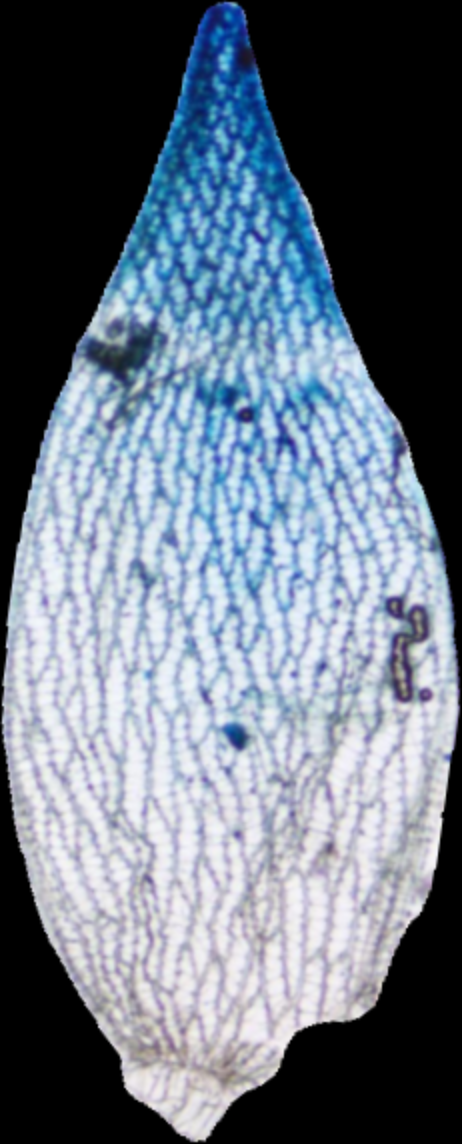
\includegraphics[height=2.8cm]{figures/121_170_0035_leaf_crop_0002.png} \\[2pt]
        {\footnotesize (а) исходное} & &
        {\footnotesize (б) маска} & &
        {\footnotesize (в) фрагмент} \\
    \end{tabular}
    \caption{Преобразование листа в конвейере: исходное изображение $\to$ очищенная
    маска $\to$ канонизированный фрагмент}
    \label{fig:pipeline_stages}
\end{figure}

Канонизация реализована в модуле \texttt{leaf\_pipeline.py} и состоит из двух шагов.

\textbf{Шаг 1: очистка маски (\texttt{preprocess\_mask}).} Реализация: поиск
всех внешних контуров через \texttt{cv2.findContours}, выбор контура максимальной
площади и заполнение получившейся области через \texttt{cv2.drawContours} с
флагом \texttt{FILLED}. На выходе~--- маска \texttt{uint8} (0 либо 255),
содержащая ровно одну связную компоненту без дыр.

\textbf{Шаг 2: канонизация ориентации (\texttt{pca\_crop}).} Ориентация листа
определяется методом главных компонент (Principal Component Analysis,
PCA)~\cite{Jolliffe2002}: по координатам активных пикселей маски строится
матрица ковариации $2 \times 2$, её собственные векторы вычисляются через
\texttt{np.linalg.eigh}. Собственный вектор с наибольшим собственным значением
указывает направление наибольшего разброса пикселей листа~--- то есть его
удлинённую (главную) ось. Изображение с обнулённым фоном поворачивается
аффинным преобразованием так, чтобы главная ось совпадала с вертикалью. После
поворота определяется направление апекса: если в верхней половине bbox больше
активных пикселей, чем в нижней, изображение переворачивается по вертикали~---
так апекс всегда оказывается сверху. Финальный шаг~--- обрезка по плотному
bounding box активных пикселей; выходом является RGB-фрагмент, в котором лист
занимает почти всю площадь и ориентирован вертикально.

\subsection{Параметрические измерения листа}
\label{sec:measure}

\subsubsection*{Алгоритм измерений}

Модуль \texttt{leaf\_measure.py} принимает на вход RGB-фрагмент в каноническом
виде (раздел~\ref{sec:pipeline}): главная ось вертикальна, апекс сверху,
фон обнулён. Это позволяет отказаться от повторного построения контура и
анализа главных компонент: все измерения сводятся к работе с маской активных
пикселей в системе координат самого фрагмента (рис.~\ref{fig:measurement}).

\begin{figure}[H]
    \centering
    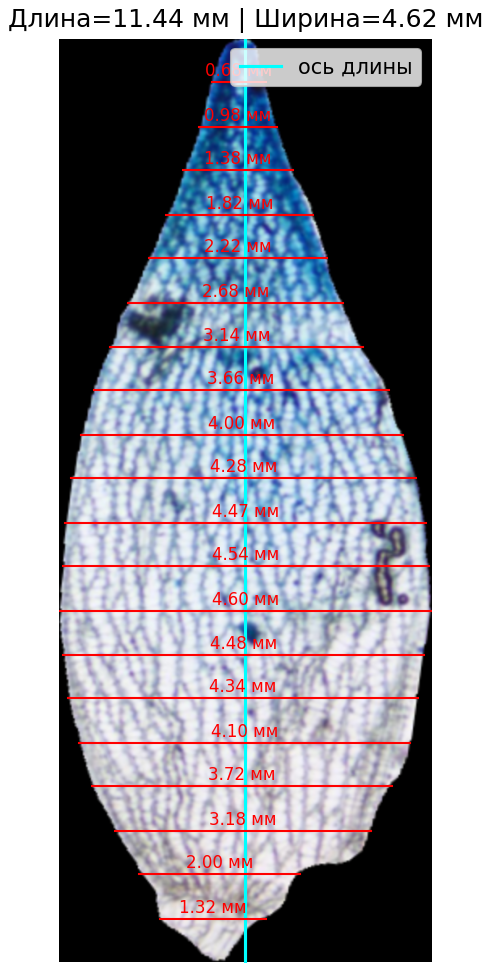
\includegraphics[width=0.22\linewidth]{figures/metrics_visualization.png}
    \caption{Визуализация измерений одного листа: длина и семь поперечных сечений}
    \label{fig:measurement}
\end{figure}

\textbf{Длина и максимальная ширина.} Длина листа определяется как высота
прямоугольника, ограничивающего активные пиксели фрагмента: $L = (y_{\max} - y_{\min} + 1) \cdot s$,
где $s$~--- масштабный коэффициент (мм/пиксель), равный единице, если пользователь
работает в пикселях. Максимальная ширина~--- ширина того же прямоугольника:
$W = (x_{\max} - x_{\min} + 1) \cdot s$.

\textbf{Поперечные сечения.} Для каждой доли $f \in (0, 1)$ берётся строка
$y = y_{\min} + \mathrm{round}\bigl(f \cdot (y_{\max} - y_{\min})\bigr)$. В этой
строке находятся крайний левый и крайний правый ненулевые пиксели $x_l$ и
$x_r$; ширина в сечении равна $w_f = (x_r - x_l + 1) \cdot s$. По умолчанию
используются семь сечений с долями
$0{,}125;\; 0{,}25;\; 0{,}375;\; 0{,}5;\; 0{,}625;\; 0{,}75;\; 0{,}875$, что
соответствует равномерному разбиению длины листа на восемь интервалов.

\textbf{Результат.} Метод возвращает структуру \texttt{LeafMetrics} с полями
\texttt{length}, \texttt{width} и словарём \texttt{widths: dict[float, SectionWidth]}~---
для каждой доли хранятся сама ширина и координаты крайних точек.

\subsubsection*{Режим замеров по готовым фрагментам}

Пакетный режим запускается из главного меню и используется, когда канонические
фрагменты уже подготовлены ранее: сохранены интерактивным режимом сегментации
(раздел~\ref{sec:interactive}), получены автоматическим режимом
(раздел~\ref{sec:auto_mode}) или предоставлены пользователем напрямую. Параметры
запуска задаются в диалоге настроек (рис.~\ref{fig:settings_dialog}): набор
файлов, выходная директория, число поперечных сечений, масштабный коэффициент,
формат экспорта (по умолчанию~--- CSV).

\begin{figure}[H]
    \centering
    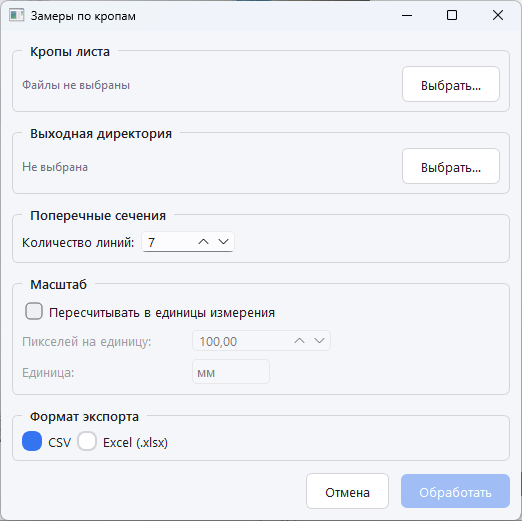
\includegraphics[width=0.6\linewidth]{figures/measure_metrics_settings_menu.png}
    \caption{Диалог настроек пакетной обработки}
    \label{fig:settings_dialog}
\end{figure}

Каждый выбранный файл читается с диска по принятой конвенции имён
(раздел~\ref{sec:architecture}) и подаётся на алгоритм измерений; результаты
по всей серии накапливаются и в конце экспортируются в таблицу. По завершении
пользователь получает диалог с числом обработанных файлов, числом ошибок и
путём к итоговой таблице. Ошибки на отдельных файлах не прерывают пакет~---
они накапливаются в результате и отображаются по окончании.

Помимо таблицы, для каждого обработанного фрагмента сохраняется изображение
\texttt{*\_vis.png} с нанесённой осью длины и поперечными сечениями
(см.\ рис.~\ref{fig:measurement}). В режиме экспорта в XLSX миниатюра этой
визуализации встраивается в ячейку таблицы, что позволяет биологу визуально
оценить корректность измерений непосредственно в Excel, не открывая файлы по
отдельности.

\subsection{Автоматическая сегментация и параметрические измерения}
\label{sec:auto_mode}

В этом режиме система обрабатывает серию изображений без участия пользователя. Конвейер обработки одного снимка состоит из пяти шагов;
на выходе всей серии~--- сводная таблица морфометрических измерений. Первые
три шага реализованы единой функцией \texttt{auto\_segment} (модуль
\texttt{leaf\_pipeline.py}).

\textbf{Шаг 1: генерация кандидатов.} Запускается \texttt{SamAutomaticMaskGenerator}.
Маски, площадь которых меньше $0{,}1\,\%$ или больше $70\,\%$ кадра,
отфильтровываются.

\textbf{Шаг 2: дедупликация.} AMG генерирует десятки масок-кандидатов; среди
них часто встречаются дубликаты~--- несколько масок одного и того же листа
разных размеров. Маски сортируются по убыванию площади и попарно отбрасываются
по порогу IoU $> 0{,}9$.

\textbf{Шаг 3: канонизация.} К каждой выжившей маске применяется конвейер
канонизации листа (раздел~\ref{sec:pipeline}). Результатом \texttt{auto\_segment}
является список пар (очищенная маска, канонический RGB-фрагмент).

\textbf{Шаг 4: фильтрация классификатором отбора.} Каждый канонический
фрагмент маркируется обученным классификатором (глава~\ref{sec:classifier_chapter})
одним из трёх классов; в итоговую таблицу попадают только фрагменты класса
\texttt{good\_leaf}.

\textbf{Шаг 5: расчёт параметров и экспорт.} К каждому отобранному фрагменту
применяется тот же алгоритм параметрических измерений, что и в режиме замеров
по готовым фрагментам (раздел~\ref{sec:measure}); результаты по всей серии
накапливаются и экспортируются в сводную таблицу. Помимо таблицы, для каждого
фрагмента сохраняются маска и канонический RGB-фрагмент в подпапках
\texttt{masks/} и \texttt{crops/} выходной директории.

Режим открывается из главного меню; диалог настроек тот же, что у режима
замеров, с одним дополнительным полем~--- выпадающим списком выбора типа листа,
по которому подгружается соответствующая модель отбора. По умолчанию формат
экспорта~--- XLSX со встроенными миниатюрами визуализаций измерений в столбце
\texttt{crop}.

\subsection{Оптимизация производительности автоматической сегментации}
\label{sec:auto_perf}

Прямолинейная реализация на ноутбуке без GPU обрабатывала один кадр $3840 \times 2160$ за
$\approx 17{,}7$~с от нажатия кнопки до отображения масок, что почти вдвое
превышает предусмотренный требованиями (раздел~\ref{sec:requirements}) бюджет в
10~с на изображение. Последовательное применение семи оптимизаций снизило это
время до $\approx 1{,}0$~с (рис.~\ref{fig:auto_perf}). Замеры выполнены на 4K-кадре с
13 масками.

\begin{figure}[H]
\centering
\begin{tikzpicture}
\definecolor{cSam}{HTML}{4E79A7}
\definecolor{cDedup}{HTML}{F28E2B}
\definecolor{cScale}{HTML}{59A14F}
\definecolor{cSave}{HTML}{E15759}
\definecolor{cClass}{HTML}{76B7B2}
\begin{axis}[
    xbar stacked,
    width=\linewidth,
    height=12.5cm,
    bar width=0.35cm,
    xmin=0, xmax=19,
    xlabel={Время, с},
    xlabel style={font=\footnotesize},
    xticklabel style={font=\footnotesize},
    xticklabel={\pgfmathprintnumber[/pgf/number format/use comma]{\tick}},
    symbolic y coords={v7,v6,v5,v4,v3,v2,v1,v0},
    ytick=\empty,
    legend style={at={(0.5,-0.12)}, anchor=north, legend columns=5,
                  font=\footnotesize, draw=none,
                  /tikz/every even column/.append style={column sep=0.5cm}},
    legend cell align=left,
    xmajorgrids,
    major grid style={dotted, gray!50},
    axis line style={draw=gray!60},
    tick style={draw=gray!60},
    enlarge y limits=0.08,
]
\addplot+[draw=none, fill=cSam]   coordinates {(6.10,v0) (0.30,v1) (0.30,v2) (0.30,v3) (0.30,v4) (0.30,v5) (0.30,v6) (0.30,v7)};
\addplot+[draw=none, fill=cDedup] coordinates {(8.54,v0) (4.99,v1) (1.17,v2) (1.16,v3) (1.17,v4) (0.93,v5) (0.28,v6) (0.28,v7)};
\addplot+[draw=none, fill=cScale] coordinates {(0.00,v0) (0.00,v1) (2.89,v2) (0.69,v3) (0.10,v4) (0.10,v5) (0.10,v6) (0.10,v7)};
\addplot+[draw=none, fill=cClass] coordinates {(0.15,v0) (0.15,v1) (0.15,v2) (0.15,v3) (0.15,v4) (0.15,v5) (0.15,v6) (0.15,v7)};
\addplot+[draw=none, fill=cSave]  coordinates {(2.89,v0) (2.86,v1) (2.84,v2) (2.89,v3) (2.90,v4) (2.90,v5) (1.62,v6) (0.17,v7)};
\legend{SAM, дедупликация, масштабирование, классификатор, сохранение}
% Подписи шагов над барами
\node[anchor=south west, font=\footnotesize, yshift=4pt] at (axis cs:0,v0) {0. Исходная реализация};
\node[anchor=south west, font=\footnotesize, yshift=4pt] at (axis cs:0,v1) {1. Понижение разрешения для сегментации};
\node[anchor=south west, font=\footnotesize, yshift=4pt] at (axis cs:0,v2) {2. Понижение разрешения для дедупликации};
\node[anchor=south west, font=\footnotesize, yshift=4pt] at (axis cs:0,v3) {3. Сокращение копирования при масштабировании};
\node[anchor=south west, font=\footnotesize, yshift=4pt] at (axis cs:0,v4) {4. Однократная канонизация};
\node[anchor=south west, font=\footnotesize, yshift=4pt] at (axis cs:0,v5) {5. Локальный IoU при дедупликации};
\node[anchor=south west, font=\footnotesize, yshift=4pt] at (axis cs:0,v6) {6. Сокращение копирования при дедупликации};
\node[anchor=south west, font=\footnotesize, yshift=4pt] at (axis cs:0,v7) {7. Асинхронное сохранение};
% Итоги справа от баров
\node[anchor=west, font=\scriptsize\bfseries] at (axis cs:17.68,v0) {17{,}7};
\node[anchor=west, font=\scriptsize\bfseries] at (axis cs:8.30,v1)  {8{,}3};
\node[anchor=west, font=\scriptsize\bfseries] at (axis cs:7.35,v2)  {7{,}4};
\node[anchor=west, font=\scriptsize\bfseries] at (axis cs:5.19,v3)  {5{,}2};
\node[anchor=west, font=\scriptsize\bfseries] at (axis cs:4.62,v4)  {4{,}6};
\node[anchor=west, font=\scriptsize\bfseries] at (axis cs:4.38,v5)  {4{,}4};
\node[anchor=west, font=\scriptsize\bfseries] at (axis cs:2.45,v6)  {2{,}5};
\node[anchor=west, font=\scriptsize\bfseries] at (axis cs:1.00,v7)  {1{,}0};
\end{axis}
\end{tikzpicture}
\caption{Время одного 4K-кадра в конвейере автоматической сегментации по шагам
оптимизации}
\label{fig:auto_perf}
\end{figure}

Семь шагов из диаграммы группируются в пять приёмов.

\textbf{Понижение входного разрешения} (шаги~1--2). Кодировщик SAM
принудительно приводит вход к квадрату $1024 \times 1024$, поэтому стоимость
самого инференса от исходного разрешения не зависит, но пост-обработка масок
(немаксимальное подавление, фильтрация по \texttt{stability\_score})
масштабируется как $O(W \cdot H \cdot N)$. Подача на вход AMG вдвое
уменьшенной копии кадра ускорила сегментацию приблизительно в 13 раз.
Аналогично, дедупликация и канонизация выполняются на той же уменьшенной
копии~--- до финального масштабирования выживших масок к исходному
разрешению,~--- что сократило время дедупликации приблизительно в 4 раза.

\textbf{Сокращение копирования кадра} (шаги~3, 6). В двух циклах~--- финальном
масштабировании и канонизации внутри дедупликации~--- для каждой маски
выполнялась полная копия кадра ($\approx 25$~МБ для исходного разрешения и
$\approx 6$~МБ для уменьшенной копии), после чего пиксели вне маски обнулялись.
Замена на копирование только области, ограниченной маской, устранила сотни
мегабайт лишних данных и существенно ускорила аффинные преобразования.

\textbf{Локальный IoU при дедупликации} (шаг~5). Изначально попарный IoU между
двумя масками считался в лоб: \texttt{logical\_and} и \texttt{logical\_or} по
всем $H \times W$ пикселям обеих масок~--- два полных прохода на каждую пару
при $\sim 17$ масках-кандидатах. Замена устроена в два шага. Во-первых, перед
попарным сравнением проверяется пересечение ограничивающих прямоугольников
масок: если прямоугольники не пересекаются, маски заведомо не пересекаются и
$\text{IoU} = 0$~--- пара отсеивается без единого пиксельного сравнения.
Во-вторых, для пересекающихся прямоугольников \texttt{logical\_and} вычисляется
только в области их пересечения, а объединение~--- по формуле
$|A \cup B| = |A| + |B| - |A \cap B|$ из заранее посчитанных площадей и только
что найденного пересечения, без второго полного прохода.

\textbf{Однократная канонизация} (шаг~4). Дедупликация уже выполняла
канонизацию каждого выжившего листа на уменьшенной копии кадра, а финальный
цикл масштабирования игнорировал этот результат и канонизировал тот же лист
повторно на полном разрешении. Замена на билинейное масштабирование уже
канонизированного фрагмента к нужному размеру избавила от двойной работы.
Возникающее размытие в~2--3 пикселя некритично.

\textbf{Асинхронное сохранение} (шаг~7). Запись масок на диск синхронно с
интерфейсом давала $\approx 2{,}9$~с зависания. Запись вынесена в фоновый пул
потоков; для отрисовки миниатюр $128 \times 128$ один раз на изображение
строится уменьшенная копия исходника ($\approx 250$~КБ вместо 25~МБ), из которой
и берутся все иконки. Интерфейс больше не блокируется на сохранение, а
синхронизация с фоновыми записями выполняется только там, где она действительно
нужна: при сохранении результатов и выходе из окна ждём завершения всех записей
перед копированием файлов в выходную папку, а при редактировании или удалении
уже сохранённой маски ждём её конкретной записи, чтобы перечитать файл с диска.

\textbf{Итог.} Время обработки одного 4K-кадра сократилось с 17{,}7 до
1{,}0~с~--- примерно в восемнадцать раз. Кнопка авто-сегментации в окне
интерактивной разметки (раздел~\ref{sec:interactive}) теперь отрабатывает за
секунду: задержка приемлема для интерактивного использования.

\subsection{Тестирование}
\label{sec:testing}

Все тесты исполняются автоматически
при каждом пуше через GitHub~Actions; внешние тяжёлые зависимости
(MobileSAM, XGBoost-модели классификатора) подменяются заглушками, что
позволяет CI работать без GPU и без модельных весов.

\textbf{Модульные тесты} ($\approx 160$ случаев) покрывают чистые функции
ядра: конвенцию имён артефактов, чтение изображений и русское склонение,
препроцессинг маски и PCA-канонизацию, API измерителя, экспорт CSV/XLSX,
конвейер обработки и адаптеры классификатора. Граничные случаи
(пустая маска, одна компонента из нескольких, дыры в маске, отсутствие
пикселей листа в выбранной строке) выделены в отдельные параметризованные
сценарии.

\textbf{Контроль точности измерений} (категория~1) выполняется на
контрольной выборке из 9 снимков, для которых эксперт-биолог вручную
замерил длину листа и семь поперечных ширин в пикселях. Тест загружает
изображение и заранее подготовленную маску, прогоняет
\texttt{transform\_leaf} и \texttt{measure\_leaf}, сверяет результат
с эталоном по критерию $\max(\delta_{\text{отн}}, \delta_{\text{абс}})$:
для длины~--- $3\,\%$, для сечений~--- $5\,\%$.

\textbf{Регрессия автосегментации} (категория~2) использует подход
\emph{golden master}: для каждого снимка контрольной выборки сохранены
площадь и центр масс всех масок, выданных текущей версией
\texttt{auto\_segment}. При повторных прогонах допускается отклонение
площади до $2\,\%$ и центра~--- до $5$~пикселей. Тест ловит регрессии
при оптимизациях конвейера, но не претендует на абсолютную меру
качества сегментации, поскольку эталон сгенерирован самим алгоритмом.

\subsection{Сборка и публикация}
\label{sec:packaging}

Целевая аудитория~--- сотрудники биологической лаборатории, для которых
установка Python и его зависимостей не является штатной операцией. Доставка
реализована в виде автономной сборки под Windows~64 на базе PyInstaller~6.11.1
в режиме \texttt{-{}-onedir}, включающей интерпретатор Python, все библиотеки и
веса моделей. Сборка использует только CPU и не требует ни предустановленного
Python, ни системных зависимостей, ни GPU.

Итоговая сборка занимает $\approx 920$~МБ и распространяется в виде
RAR-архива ($\approx 327$~МБ); готовые сборки опубликованы в разделе
\href{https://github.com/pavelrubanov/segmentation_system/releases}{Releases}
репозитория проекта. Запуск~--- двойным кликом по \texttt{sphagnum.exe};
стандартные потоки перенаправляются в файлы \texttt{stdout.log} и
\texttt{stderr.log} в её директории.


% !TeX spellcheck = ru_RU
% !TEX root = vkr.tex

\section{Обучение классификатора отбора листьев}
\label{sec:classifier_chapter}

\subsection{Постановка задачи}
\label{sec:classifier_task}

После сегментации (раздел~\ref{sec:auto_mode}) получается набор
масок-кандидатов всех объектов на изображении: и корректные одиночные
листья, пригодные для измерений, и брак~--- повреждённые, перекрывающиеся,
нелистовые артефакты. Для отбора пригодных листьев обучается отдельный
классификатор. Вход модели~--- канонический RGB-фрагмент
(раздел~\ref{sec:pipeline}). Выход~--- метка одного из трёх классов:

\begin{itemize}
    \item \texttt{good\_leaf}~--- корректный одиночный лист, пригодный для
          морфометрических измерений;
    \item \texttt{bad\_leaf}~--- лист с дефектами (перекрытия с другими
          объектами, неполная форма, рваные края);
    \item \texttt{non\_leaf}~--- объект нелистовой природы (фон, тень,
          артефакт сегментации).
\end{itemize}

Стоимость ошибок классификатора несимметрична: пропущенный лист
безвозвратно теряется, тогда как ложно положительный фрагмент попадает в
итоговую таблицу измерений и удаляется вручную. Поэтому в качестве рабочей
точки фиксируется уровень recall $\geq 0{,}95$ на позитивном классе
\texttt{good\_leaf}~--- гарантия, что не более $\sim 5\,\%$ корректных
листьев теряется на этапе фильтрации. Соответствующая precision при этом
recall используется как основная метрика качества по всей главе.

\subsection{Архитектура классификатора}
\label{sec:classifier}

Малый объём ручной разметки ($\sim 100\!-\!600$ позитивных примеров на тип
листа, см.\ табл.~\ref{tab:clf_balance}) исключает дообучение свёрточной сети
целиком~--- риск переобучения слишком высок. Поэтому классификатор реализован
как двухэтапная модель: замороженный экстрактор признаков на основе свёрточной
сети, предобученной на ImageNet, и градиентный бустинг XGBoost, обучаемый на
этих признаках (рис.~\ref{fig:classifier_pipeline}).

\begin{figure}[H]
    \centering
    \begin{tikzpicture}[
        font=\scriptsize,
        box/.style={rectangle, draw, rounded corners=2pt,
                    minimum height=1.5cm, align=center, fill=gray!4,
                    inner sep=4pt},
        arr/.style={->, >=Stealth, thick},
        node distance=0.45cm,
    ]
    \node[inner sep=0pt] (img)
        {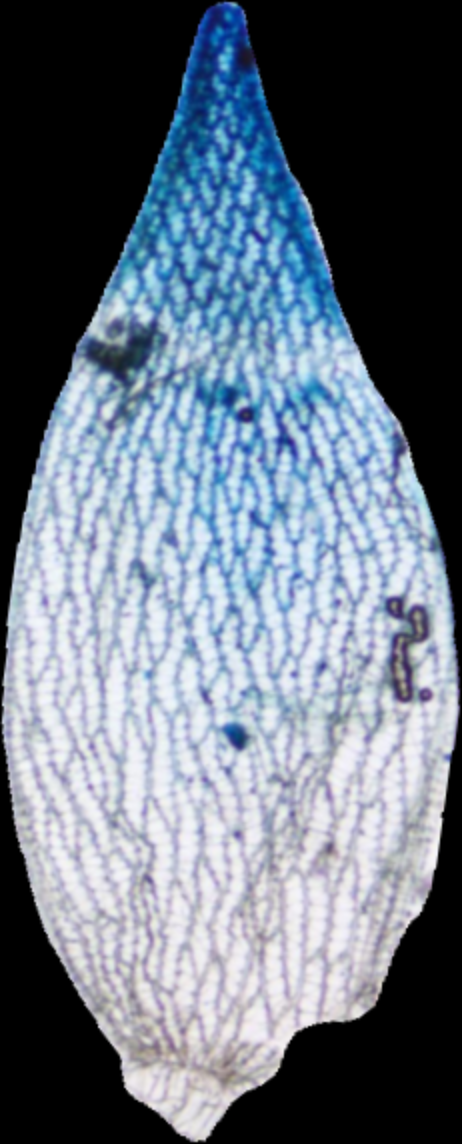
\includegraphics[height=1.9cm]{figures/121_170_0035_leaf_crop_0002.png}};
    \node[inner sep=0pt, right=of img] (letter)
        {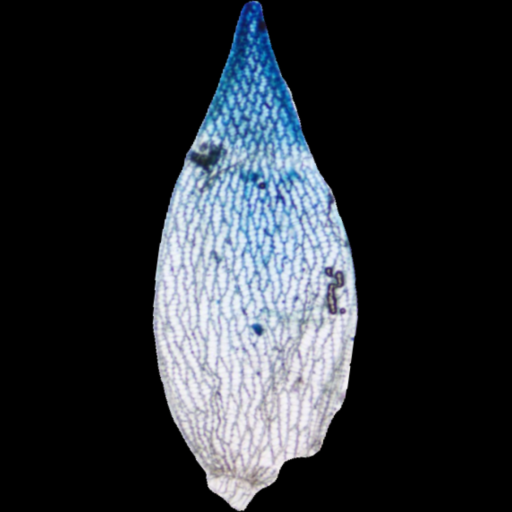
\includegraphics[height=1.9cm]{figures/121_170_0035_leaf_crop_0002_letterbox.png}};
    \node[box, right=of letter, minimum width=2.6cm, fill=blue!8] (mnet)
        {MobileNetV3-Small\\(заморожена)};
    \node[box, right=of mnet, minimum width=1.7cm] (feat)
        {576\\признаков};
    \node[box, right=of feat, minimum width=2.4cm, fill=orange!10] (xgb)
        {XGBoost\\300 деревьев};
    \node[box, right=of xgb, minimum width=1.9cm] (out)
        {\texttt{good\_leaf}\\\texttt{bad\_leaf}\\\texttt{non\_leaf}};
    \foreach \a/\b in {img/letter, letter/mnet, mnet/feat, feat/xgb, xgb/out}
        \draw[arr] (\a.east) -- (\b.west);
    \end{tikzpicture}
    \caption{Конвейер классификатора отбора масок}
    \label{fig:classifier_pipeline}
\end{figure}

\subsubsection*{Извлечение признаков}

Используется MobileNetV3-Small из \texttt{torchvision}, предобученная на
ImageNet. Финальный классификационный слой заменяется на \texttt{Identity}
(сеть возвращает 576-мерный эмбеддинг вместо 1000 ImageNet-логитов), все
параметры заморожены. Каждый фрагмент
вписывается в квадрат $512 \times 512$ пикселей с сохранением пропорций, нормализуется по статистикам ImageNet
и пропускается через сеть; на выходе~--- вектор $576$ признаков.

\subsubsection*{Параметры XGBoost}

XGBoost (\texttt{XGBClassifier}, \texttt{multi:softprob}) с гиперпараметрами:
$300$ деревьев, максимальная глубина $6$, темп обучения $0{,}1$,
\texttt{subsample}$\,= 0{,}8$, \texttt{colsample\_bytree}$\,= 0{,}8$,
\texttt{tree\_method}$\,=$ \texttt{"hist"}. Веса классов компенсируют
дисбаланс ($\sim 100\!-\!600$ позитивных против $1500$ \texttt{bad\_leaf} и
$\sim 1000$ \texttt{non\_leaf}) и задаются формулой:
\begin{equation}
    w_c = \frac{N_{\text{total}}}{n_{\text{classes}} \cdot N_c},
    \label{eq:class_weights}
\end{equation}
где $N_c$~--- число примеров класса~$c$, $N_{\text{total}}$~--- общий размер
обучающей выборки. Обоснование выбора численных значений приведено в
разделе~\ref{sec:classifier_justification}.

\subsection{Сбор обучающей выборки}
\label{sec:classifier_dataset}

Размеченная выборка собрана автором работы с использованием интерактивного
режима приложения (раздел~\ref{sec:interactive}): на каждом исходном снимке
запускалась автосегментация, полученные кандидаты вручную распределялись по
трём классам.

Морфология листьев у разных групп \textit{Sphagnum} существенно различается, поэтому
позитивный класс \texttt{good\_leaf\_<type>} собран отдельно для каждого из
трёх типов, а отказные классы \texttt{bad\_leaf} (повреждённые или перекрытые
листья) и \texttt{non\_leaf} (артефакты сегментации, фон, тени)~--- общие для
всех типов и не требуют повторной разметки. Полный датасет
опубликован: \url{https://cloud.mail.ru/public/jvB9/ReNV4TrpS}.

\begin{table}[H]
\centering
\caption{Распределение классов в обучающей выборке (по типам листа)}
\label{tab:clf_balance}
\small
\begin{tabular}{lcccc}
\hline
\textbf{Тип листа} & \texttt{good\_leaf} & \texttt{bad\_leaf} & \texttt{non\_leaf} & \textbf{Доля \texttt{good}} \\
\hline
\texttt{branch}        & 566  & 1500 & 994  & $18{,}5\,\%$ \\
\texttt{capillifolium} & 121  & 1500 & 994  & $4{,}6\,\%$  \\
\texttt{girgensohnii}  & 309  & 1500 & 994  & $11{,}0\,\%$ \\
\hline
\end{tabular}
\end{table}

\subsubsection*{Аугментация}

Каждый фрагмент размножается в шесть детерминированных вариантов: горизонтальное
отражение (два состояния), перемноженное на три цветовые трансформации~---
оригинал, осветление и затемнение по яркости, контрасту и насыщенности.
Вертикальное отражение нарушило бы инвариант ``апекс сверху'' и не
используется. Признаки MobileNetV3 вычисляются для каждого варианта один раз
и кэшируются.

\subsection{Результаты}
\label{sec:classifier_results}

Качество оценивается $5$-кратной стратифицированной кросс-валидацией; на
обучающих разбиениях применяется шестикратная аугментация, тестовое
разбиение проходит без аугментации. По накопленным предсказаниям пяти
разбиений в бинарной задаче \texttt{good\_leaf} против объединения
\texttt{bad\_leaf} и \texttt{non\_leaf} для каждого типа листа найден
минимальный порог $p_{\text{good}}$, при котором recall $\geq 0{,}95$
(рис.~\ref{fig:clf_pr_curve}).

\begin{figure}[H]
    \centering
    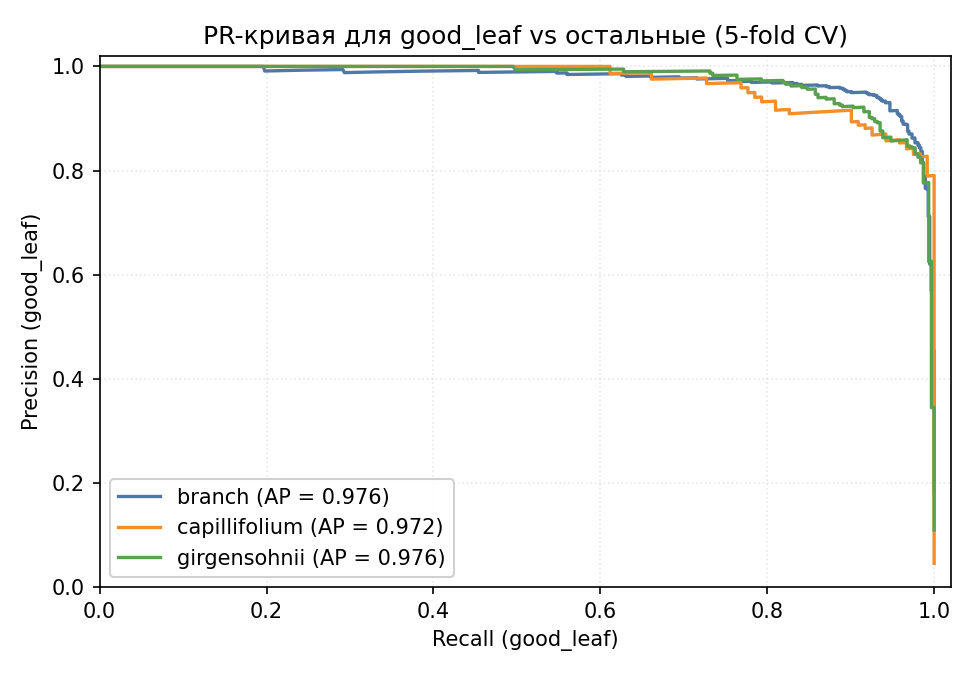
\includegraphics[width=0.6\linewidth]{figures/classifier_pr_curve.png}
    \caption{PR-кривая классификатора для бинарной задачи
    \texttt{good\_leaf} против остальных классов (5-кратная
    кросс-валидация)}
    \label{fig:clf_pr_curve}
\end{figure}

\begin{table}[H]
\centering
\caption{Метрики классификатора на рабочей точке recall $\geq 0{,}95$
(5-кратная кросс-валидация)}
\label{tab:clf_metrics}
\small
\begin{tabular}{lccccc}
\hline
\textbf{Тип листа} & $\boldsymbol{p_{\text{good}}}$ &
\textbf{Precision} & \textbf{Recall} & \textbf{F1} & \textbf{AP} \\
\hline
\texttt{branch}        & $0{,}22$ & $0{,}921 \pm 0{,}027$ & $0{,}95$ & $0{,}935$ & $0{,}977 \pm 0{,}009$ \\
\texttt{capillifolium} & $0{,}24$ & $0{,}884 \pm 0{,}050$ & $0{,}95$ & $0{,}916$ & $0{,}972 \pm 0{,}014$ \\
\texttt{girgensohnii}  & $0{,}12$ & $0{,}882 \pm 0{,}049$ & $0{,}95$ & $0{,}915$ & $0{,}978 \pm 0{,}009$ \\
\hline
\end{tabular}
\end{table}

Precision и AP даны как среднее по 5 фолдам $\pm$ стандартное отклонение
между фолдами. На всех трёх типах достигнут целевой recall при precision
$0{,}88\!-\!0{,}92$. Площадь под PR-кривой $> 0{,}97$ для всех типов
означает, что модель хорошо разделяет позитивный класс почти на всём
диапазоне порогов. Минимальная precision на \texttt{capillifolium} и
\texttt{girgensohnii} связана с меньшим объёмом размеченных позитивных
примеров ($121$ и $309$ против $566$ для \texttt{branch}).

Разброс по фолдам ($\pm 2{,}7$\,п.п.\ на \texttt{branch}, $\pm 5$\,п.п.\
на \texttt{capillifolium} и \texttt{girgensohnii}) при усреднении по 5
разбиениям даёт стандартную ошибку среднего
$\sigma_{\text{CV}} \approx 1\!-\!2$\,п.п.~--- этим определяется уровень
шума при сравнении архитектурных вариантов в
разделе~\ref{sec:classifier_justification}.

\subsection{Сравнение с альтернативными архитектурами}
\label{sec:classifier_justification}

Каждое архитектурное решение проверено отдельным экспериментом по тому же
протоколу 5-кратной кросс-валидации, что и в табл.~\ref{tab:clf_metrics};
метрика~--- precision при recall $= 0{,}95$ на классе \texttt{good\_leaf}. Прикладные ограничения, принимаемые во внимание при
выборе архитектуры: вычисления на CPU рабочей станции лаборатории, малый
объём ручной разметки ($\sim 100\!-\!600$ позитивных примеров на тип листа),
повторное обучение силами лаборатории при добавлении нового типа.

\subsubsection*{Выбор сети-экстрактора признаков}

Сравнивались восемь замороженных экстракторов признаков с фиксированным
итоговым классификатором XGBoost (табл.~\ref{tab:clf_backbones}).

\begin{table}[H]
\centering
\caption{Precision при recall $= 0{,}95$ для разных экстракторов признаков}
\label{tab:clf_backbones}
\scriptsize
\begin{tabular}{lcccrr}
\hline
\textbf{Экстрактор} & \textbf{branch} & \textbf{capilli.} & \textbf{girgens.} &
\textbf{CPU,\,мс} & \textbf{Вес,\,МБ} \\
\hline
\textbf{MobileNetV3-Small (выбран)} & $\mathbf{0{,}913 \pm 0{,}049}$ & $\mathbf{0{,}896 \pm 0{,}039}$ & $0{,}889 \pm 0{,}030$ & $\mathbf{6}$ & $\mathbf{9{,}7}$ \\
EfficientNet-B0    & $0{,}901 \pm 0{,}038$ & $0{,}826 \pm 0{,}048$ & $0{,}904 \pm 0{,}027$ & $13$  & $20{,}5$ \\
DINOv2-small       & $0{,}882 \pm 0{,}035$ & $\mathbf{0{,}896 \pm 0{,}109}$ & $\mathbf{0{,}911 \pm 0{,}029}$ & $192$ & $84{,}2$ \\
MobileNetV3-Large  & $0{,}874 \pm 0{,}006$ & $0{,}841 \pm 0{,}062$ & $0{,}877 \pm 0{,}044$ & $16$  & $21{,}0$ \\
ResNet-50          & $0{,}896 \pm 0{,}015$ & $0{,}875 \pm 0{,}108$ & $0{,}889 \pm 0{,}013$ & $25$  & $97{,}8$ \\
ConvNeXt-Tiny      & $0{,}879 \pm 0{,}044$ & $0{,}857 \pm 0{,}034$ & $0{,}898 \pm 0{,}020$ & $25$  & $109{,}1$ \\
ResNet-18          & $0{,}872 \pm 0{,}027$ & $0{,}740 \pm 0{,}142$ & $0{,}886 \pm 0{,}046$ & $11$  & $44{,}7$ \\
MobileSAM-encoder  & $0{,}772 \pm 0{,}069$ & $0{,}686 \pm 0{,}081$ & $0{,}801 \pm 0{,}036$ & $347$ & $38{,}8$ \\
\hline
\end{tabular}
\end{table}

MobileNetV3-Small лидирует на \texttt{branch} (самой крупной выборке) и
\texttt{capillifolium}, на \texttt{girgensohnii} уступает DINOv2-small на
$2{,}2$\,п.п.~--- в пределах CV-шума $\sigma_{\text{CV}}$. DINOv2
проигрывает в $32$ раза по скорости и в $8{,}7$ раза по объёму весов~---
неприемлемо для рабочей станции без GPU. Кодировщик MobileSAM
(переиспользование весов сегментатора) даёт просадку
$8{,}8\!-\!21{,}0$\,п.п.\ при $58$-кратном замедлении~--- разрыв
кратно превышает шум, эта замена однозначно отвергается.

\subsubsection*{Сравнение глубоких и ручных признаков}

Морфометрическая базовая модель на $84$ ручных признаках (форма и площадь,
профиль ширины, эллиптические Фурье-дескрипторы, моменты Ху, симметрия,
кривизна у апекса) с тем же XGBoost сравнена с признаками MobileNet
(табл.~\ref{tab:clf_features}).

\begin{table}[H]
\centering
\caption{Precision при recall $= 0{,}95$: глубокие и ручные признаки}
\label{tab:clf_features}
\small
\begin{tabular}{lccc}
\hline
\textbf{Признаки} & \textbf{branch} & \textbf{capilli.} & \textbf{girgens.} \\
\hline
\textbf{MobileNetV3-Small (576-d, выбран)} & $\mathbf{0{,}913 \pm 0{,}049}$ & $\mathbf{0{,}896 \pm 0{,}039}$ & $\mathbf{0{,}889 \pm 0{,}030}$ \\
$84$ ручных & $0{,}793 \pm 0{,}074$ & $0{,}577 \pm 0{,}159$ & $0{,}616 \pm 0{,}052$ \\
\hline
\end{tabular}
\end{table}

Разрыв $12{,}0\!-\!31{,}9$\,п.п.\ означает, что контурная геометрия не
описывает текстурный сигнал, существенный для отбраковки повреждённых и
нелистовых объектов.

\subsubsection*{Выбор классификатора}

На зафиксированных признаках MobileNet сравнивались шесть альтернатив XGBoost
(табл.~\ref{tab:clf_models}).

\begin{table}[H]
\centering
\caption{Precision при recall $= 0{,}95$ для разных классификаторов поверх
признаков MobileNetV3-Small}
\label{tab:clf_models}
\small
\begin{tabular}{lccc}
\hline
\textbf{Модель} & \textbf{branch} & \textbf{capilli.} & \textbf{girgens.} \\
\hline
\textbf{XGBoost (выбран)} & $\mathbf{0{,}921 \pm 0{,}027}$ & $0{,}884 \pm 0{,}050$ & $0{,}882 \pm 0{,}049$ \\
RBF-SVM       & $0{,}888 \pm 0{,}039$ & $0{,}906 \pm 0{,}052$ & $\mathbf{0{,}918 \pm 0{,}036}$ \\
MLP           & $0{,}892 \pm 0{,}037$ & $\mathbf{0{,}911 \pm 0{,}059}$ & $0{,}897 \pm 0{,}025$ \\
LogReg        & $0{,}860 \pm 0{,}050$ & $0{,}876 \pm 0{,}093$ & $0{,}845 \pm 0{,}039$ \\
RandomForest  & $0{,}862 \pm 0{,}035$ & $0{,}717 \pm 0{,}096$ & $0{,}873 \pm 0{,}049$ \\
LinearSVM     & $0{,}814 \pm 0{,}015$ & $0{,}822 \pm 0{,}064$ & $0{,}877 \pm 0{,}034$ \\
kNN           & $0{,}801 \pm 0{,}056$ & $0{,}749 \pm 0{,}092$ & $0{,}821 \pm 0{,}052$ \\
\hline
\end{tabular}
\end{table}

XGBoost~--- лидер на \texttt{branch} (самой крупной выборке); на
\texttt{capillifolium} и \texttt{girgensohnii} он уступает MLP и RBF-SVM
на $2{,}7\!-\!3{,}6$\,п.п.~--- порядка $1\!-\!2\,\sigma_{\text{CV}}$, на
грани шума и без устойчивого преимущества альтернатив. XGBoost оставлен
как лидер на самой крупной выборке плюс встроенная поддержка
\texttt{sample\_weight} для компенсации дисбаланса. Линейные модели
(LogReg, LinearSVM) и kNN отстают на $5\!-\!10$\,п.п.~--- разрыв
кратно превышает шум.

\subsubsection*{Параметры XGBoost}

Для проверки выбранных значений и оценки, нужна ли отдельная подстройка
под каждый тип листа, выполнен поиск по сетке (\texttt{n\_estimators}
$\in [50;\,1500]$, \texttt{max\_depth} $\in [2;\,12]$,
\texttt{learning\_rate} $\in [0{,}01;\,0{,}3]$, \texttt{subsample},
\texttt{colsample\_bytree} $\in [0{,}5;\,1{,}0]$): каждый параметр
перебирался независимо при остальных, зафиксированных на выбранных
значениях.

\begin{figure}[H]
\centering
\begin{tikzpicture}
\begin{axis}[
    width=0.85\linewidth, height=6.5cm,
    xlabel={Число деревьев $n_{\text{est}}$},
    ylabel={precision при recall $= 0{,}95$},
    xmin=0, xmax=1280,
    ymin=0.82, ymax=0.93,
    legend style={at={(0.98,0.04)}, anchor=south east, font=\footnotesize,
                  draw=gray!50, fill=white, fill opacity=0.85,
                  text opacity=1},
    legend cell align={left},
    grid=major, grid style={dashed,gray!25},
    tick label style={font=\footnotesize},
    label style={font=\footnotesize},
    mark size=1.4pt,
]
\addplot[mark=*, color=blue!70!black, thick] coordinates {
    (50, 0.8911) (100, 0.8997) (150, 0.9139) (200, 0.9193)
    (300, 0.9208) (500, 0.9163) (800, 0.9161) (1200, 0.9147)
};
\addlegendentry{\texttt{branch}}
\addplot[mark=square*, color=red!70!black, thick] coordinates {
    (50, 0.8259) (100, 0.8574) (150, 0.8757) (200, 0.8761)
    (300, 0.8838) (500, 0.8969) (800, 0.8975) (1200, 0.8975)
};
\addlegendentry{\texttt{capillifolium}}
\addplot[mark=triangle*, color=green!50!black, thick] coordinates {
    (50, 0.8659) (100, 0.8665) (150, 0.8717) (200, 0.8751)
    (300, 0.8816) (500, 0.8841) (800, 0.8841) (1200, 0.8860)
};
\addlegendentry{\texttt{girgensohnii}}
\draw[dashed, gray!70, thick]
    (axis cs:300,0.82) -- (axis cs:300,0.93);
\node[gray!80, font=\footnotesize, anchor=south]
    at (axis cs:300,0.82) {\,300};
\end{axis}
\end{tikzpicture}
\caption{Зависимость precision (при recall $= 0{,}95$) от числа деревьев
XGBoost при остальных параметрах, фиксированных на выбранных значениях.
Пунктир~--- выбранное $n_{\text{est}} = 300$.}
\label{fig:clf_xgb_curve}
\end{figure}

На \texttt{branch} (самой крупной выборке) выбранные значения уже стоят
в максимуме сетки по всем пяти параметрам~--- одиночное изменение любого
из них только ухудшает precision. На меньших выборках
\texttt{capillifolium} и \texttt{girgensohnii} лучший прирост от
изменения одного параметра не превышает $2$\,п.п., что не выходит за
шум $\sigma_{\text{CV}}$. Лучшие значения по разным типам листа взаимно
противоречат (например, \texttt{max\_depth}: $6$ / $4$ / $5$;
\texttt{subsample}: $0{,}8$ / $0{,}7$ / $1{,}0$)~--- характерное
проявление переобучения на конкретные разбиения, а не сигнал о наличии
предпочтительной конфигурации под отдельный тип. Поэтому единая
конфигурация $(\texttt{n\_estimators} = 300$, $\texttt{max\_depth} = 6$,
$\texttt{learning\_rate} = 0{,}1$, $\texttt{subsample} = 0{,}8$,
$\texttt{colsample\_bytree} = 0{,}8)$ оставлена для всех трёх моделей.

\subsubsection*{Число классов}

Бинарная постановка (\texttt{good} против объединения \texttt{bad} и
\texttt{non}) проверена на той же выборке и том же XGBoost
(табл.~\ref{tab:clf_classes}).

\begin{table}[H]
\centering
\caption{Precision при recall $= 0{,}95$: трёхклассовая и бинарная постановка}
\label{tab:clf_classes}
\small
\begin{tabular}{lccc}
\hline
\textbf{Постановка} & \textbf{branch} & \textbf{capilli.} & \textbf{girgens.} \\
\hline
\textbf{3 класса (выбрана)} & $\mathbf{0{,}921 \pm 0{,}027}$ & $\mathbf{0{,}884 \pm 0{,}050}$ & $0{,}882 \pm 0{,}049$ \\
2 класса (\texttt{good} против остального) & $0{,}895 \pm 0{,}042$ & $0{,}839 \pm 0{,}051$ & $\mathbf{0{,}896 \pm 0{,}044}$ \\
\hline
\end{tabular}
\end{table}

3-классовая постановка выигрывает на \texttt{branch} ($+2{,}6$\,п.п.) и
\texttt{capillifolium} ($+4{,}5$\,п.п., $\sim 2\sigma_{\text{CV}}$), уступает
на \texttt{girgensohnii} ($-1{,}5$\,п.п., в пределах $\sigma_{\text{CV}}$).
На самом малом позитивном классе (\texttt{capillifolium}, $121$ образец)
разрыв максимальный~--- различение типов отказа даёт дополнительный
обучающий сигнал, особенно ценный при малом числе положительных примеров.

\subsubsection*{Итог раздела}

Главный ограничитель качества классификатора~--- объём и качество
размеченной выборки (\texttt{capillifolium}~--- $121$ позитивный пример,
\texttt{girgensohnii}~--- $309$, табл.~\ref{tab:clf_balance}), а не
архитектурные решения: расширение и уточнение разметки сдвинут рабочую
точку существеннее любой замены сети-экстрактора, классификатора или
подстройки гиперпараметров.

% !TeX spellcheck = ru_RU
% !TEX root = vkr.tex

\section{Эксперимент и апробация}
\label{sec:experiment}

\subsection{Цель и методология}

Целью эксперимента является количественная оценка точности автоматических морфометрических измерений
системы путём сравнения с ручными измерениями, выполненными специалистом лаборатории Гербарий ГБС РАН.

Тестовая выборка включает 9~изображений листьев \textit{Sphagnum} трех разных типов.
Для каждого изображения специалист выполнил ручное измерение двух морфометрических характеристик:
\begin{itemize}
    \item длины листа по главной оси;
    \item поперечных профилей ширины в семи равноотстоящих сечениях
          (на долях 0.125, 0.25, 0.375, 0.5, 0.625, 0.75, 0.875 от полной длины).
\end{itemize}

Те же изображения были обработаны разработанной системой через режим автоматической сегментации и параметрических измерений.
Маски сохранены в директории \texttt{metric\_test/results/};
ручные эталонные измерения~--- в \texttt{metric\_test/mapped/}.

\subsection{Сравнение длин листьев}

В таблице~\ref{tab:lengths} приведены автоматические и ручные измерения длины для всех девяти образцов.
Все автоматические значения превышают ручные, что свидетельствует о систематическом завышении.

\begin{table}[H]
\centering
\caption{Сравнение автоматических и ручных измерений длины листа (пиксели)}
\label{tab:lengths}
\begin{tabular}{crrrr}
\hline
\textbf{№} & \textbf{Авто} & \textbf{Вручную} & $\Delta$, px & APE, \% \\
\hline
1 & 1131.9 & 1106.2 & +25.7  &  2.3 \\
2 &  734.2 &  703.2 & +31.0  &  4.4 \\
3 & 1142.9 & 1132.0 & +10.9  &  1.0 \\
4 & 1511.2 & 1446.2 & +65.0  &  4.5 \\
5 & 2018.4 & 1992.2 & +26.2  &  1.3 \\
6 &  850.9 &  766.9 & +84.0  & 11.0 \\
7 & 1899.2 & 1680.4 & +218.8 & 13.0 \\
8 &  855.2 &  829.2 & +26.0  &  3.1 \\
9 &  443.8 &  408.2 & +35.6  &  8.7 \\
\hline
\textbf{Итого} & & & \textbf{+58.1} & \textbf{5.5} \\
\hline
\end{tabular}
\end{table}

Средняя абсолютная погрешность составила MAE\,=\,58.1\,px при RMSE\,=\,84.0\,px
и средней относительной погрешности MAPE\,=\,5.5\,\%.
Коэффициент корреляции $R = 0.993$ свидетельствует о высокой линейной согласованности
автоматических и ручных измерений.

Наибольшие отклонения наблюдаются у образцов № 7 и № 6
(APE\,=\,13.0\,\% и 11.0\,\%) и объясняются субъективностью ручного измерения:
у этих образцов в основании листа имеются выросты~--- структуры,
относящиеся к листу, которые эксперт при ручной разметке решил не включать в
измеряемую длину. Алгоритм же по полной маске учитывает их как часть листа,
что и даёт расхождение. Для остальных образцов с более регулярной формой
основания относительная погрешность длины не превышает 5\,\%.

\subsection{Сравнение поперечных профилей ширины}

В таблице~\ref{tab:cross} представлены метрики погрешности для поперечных профилей
по каждому из девяти образцов. Анализ проводился по всем 63~значениям (9 листьев $\times$ 7 сечений).

\begin{table}[H]
\centering
\caption{Метрики погрешности поперечных профилей ширины (пиксели)}
\label{tab:cross}
\begin{tabular}{crrrr}
\hline
\textbf{№} & \textbf{Bias} & \textbf{MAE} & \textbf{RMSE} & \textbf{MAPE, \%} \\
\hline
1 & $-3.9$ &  7.7 & 10.7 & 1.95 \\
2 & $-3.9$ &  9.2 & 11.2 & 1.75 \\
3 & $-1.2$ &  2.3 &  2.7 & 0.60 \\
4 &$-12.9$ & 13.7 & 16.3 & 1.54 \\
5 &$-14.3$ & 14.4 & 20.8 & 2.41 \\
6 & $+7.1$ & 13.7 & 16.2 & 3.97 \\
7 &$+12.1$ & 20.7 & 25.3 & 2.44 \\
8 & $-1.8$ &  3.9 &  4.2 & 0.96 \\
9 & $-3.5$ &  4.4 &  7.1 & 1.43 \\
\hline
\textbf{Итого} & $\mathbf{-2.5}$ & \textbf{10.0} & \textbf{14.6} & \textbf{1.90} \\
\hline
\end{tabular}
\end{table}

Суммарная MAPE по поперечным профилям составила \textbf{1.90\,\%}~. Коэффициент корреляции $R = 0.998$ при 63~парах наблюдений подтверждает
высокую согласованность алгоритма сканирования поперечных сечений с ручными измерениями.

Систематический сдвиг по профилям незначителен (Bias\,=\,$-2.5$\,px) и не имеет
выраженного направления: у одних образцов алгоритм слегка занижает ширину (листья 1, 2, 4, 5),
у других~--- слегка завышает (листья 6, 7).

\subsection{Итоговые показатели}

В таблице~\ref{tab:summary} сведены итоговые метрики по двум типам измерений.

\begin{table}[H]
\centering
\small
\caption{Итоговые метрики точности автоматических измерений (Bias, MAE, RMSE~--- в пикселях)}
\label{tab:summary}
\begin{tabular}{lrrrrrr}
\hline
\textbf{Тип измерения} & $N$ & \textbf{Bias} & \textbf{MAE} & \textbf{RMSE} & \textbf{MAPE, \%} & $R$ \\
\hline
Длина листа              &  9 & $+58.1$ & 58.1 & 84.0 & 5.5  & 0.993 \\
Поперечные профили ширины& 63 &  $-2.5$ & 10.0 & 14.6 & 1.90 & 0.998 \\
\hline
\end{tabular}
\end{table}

Измерение поперечных профилей демонстрирует высокую точность~--- погрешность
менее 2\,\% приемлема для сравнительного морфометрического анализа.
Длина листа имеет систематическое завышение порядка 5--6\,\% относительно
ручных измерений: алгоритм по полной маске учитывает выросты у основания
листа, которые эксперт при ручной разметке субъективно исключает (см. анализ
образцов № 7 и № 6 выше).

\subsection{Сравнение по затратам времени}

Среднее время ручного измерения одного листа экспертом составило
$2{,}6 \pm 0{,}4$~минут; автоматическая обработка одного изображения заняла
$\approx 1{,}0$~с (раздел~\ref{sec:auto_perf}), что соответствует ускорению
приблизительно на два порядка.

\subsection{Апробация}

Прототип системы был продемонстрирован консультанту~--- м.н.с.\ лаборатории Гербарий ГБС РАН
Шкурко~А.~В. По итогам демонстрации качество автоматической сегментации признано
удовлетворительным для дальнейшего развития системы.
Видеозапись демонстрации прилагается к работе.

В ходе апробации были выявлены следующие направления доработки:
\begin{itemize}
    \item поддержка масштабного коэффициента (пересчёт пикселей в мм);
    \item возможность экспорта визуализаций в дополнение к CSV;
    \item расстановка точек вдоль периметра с заданным шагом (требование из технического задания).
\end{itemize}

% !TeX spellcheck = ru_RU
% !TEX root = vkr.tex

\section*{Заключение}
\label{sec:conclusion}

В ходе работы разработана система для автоматической сегментации и
морфометрических измерений листьев \textit{Sphagnum} в виде настольного
приложения под Windows. Были выполнены следующие задачи:

\begin{enumerate}
    \item Сформулированы требования к разрабатываемой системе.

    \item Спроектирована архитектура и реализовано приложение с тремя режимами
          работы: интерактивная сегментация, параметрические измерения по
          готовым фрагментам и автоматическая сегментация с измерениями.
          Время обработки одного 4K-кадра в автоматическом режиме~---
          $\approx 1{,}0$~с.

    \item Собрана и размечена обучающая выборка для классификатора отбора
          листьев~--- около $3500$ канонизированных фрагментов, в том числе
          $996$ корректных листьев трёх типов \textit{Sphagnum}.

    \item Обучен классификатор отбора для трёх типов листьев
          \textit{Sphagnum}; на классе \texttt{good\_leaf} при гарантированном
          recall $= 0{,}95$ precision составляет $0{,}88\!-\!0{,}92$,
          AP $> 0{,}97$.

    \item Проведено сравнение автоматических измерений с ручной разметкой
          эксперта на $9$ контрольных снимках: MAPE длины = $5{,}5\,\%$,
          MAPE поперечных профилей = $1{,}90\,\%$.
          Прототип апробирован консультантом, качество признано
          удовлетворительным.
\end{enumerate}

\textbf{Артефакты работы:}

\begin{itemize}
    \item Исходный код приложения: \\
          \url{https://github.com/pavelrubanov/segmentation_system}
    \item Размеченный датасет: \\
          \url{https://cloud.mail.ru/public/jvB9/ReNV4TrpS}
    \item Готовая сборка под Windows~64: \\
          \url{https://github.com/pavelrubanov/segmentation_system/releases}
\end{itemize}


\setmonofont{CMU Typewriter Text}
\bibliographystyle{ugost2008ls}
\bibliography{vkr}
\end{document}
